% !TEX root = ./rapport.tex
\chapter{Analyse, Conception et Choix Technologiques}

\noindent\textbf{Plan}
\begin{enumerate}
  \item Introduction
  \item Spécification des besoins
  \item Identification des acteurs
  \item Diagrammes de cas d’utilisation
  \item Architecture générale de Synapse
  \item Modélisation des données
  \item Environnement de développement
  \item Planification du projet
  \item Étude et justification des choix technologiques
  \item Conclusion
\end{enumerate}

% ─────────────────────────────────────────────────────────────
\section{Introduction}
% ─────────────────────────────────────────────────────────────

En amont de tout développement, l’analyse des besoins et la planification jouent
un rôle déterminant~: c’est là que les exigences sont formalisées, que les acteurs
sont identifiés et que les technologies sont comparées et sélectionnées. Ce chapitre
présente l’ensemble de cette démarche pour la plateforme Synapse~: spécification des
besoins fonctionnels et non fonctionnels, modélisation UML\textsuperscript{[3]}, architecture retenue,
environnement de développement, planification Scrum et justification des choix
technologiques.

% ─────────────────────────────────────────────────────────────
\section{Spécification des besoins}

\subsection{Besoins fonctionnels}

Les tableaux suivants présentent les besoins fonctionnels de Synapse organisés par acteur.

\begin{table}[H]
\centering
\caption{Besoins fonctionnels — Employé}
\label{tab:bf_employe}
\begin{tabularx}{\textwidth}{VLVlV}
\rowcolor{headerblue!55}
\hline
\textbf{Besoin fonctionnel} & \textbf{Priorité} \\
\hline
S’authentifier via Keycloak (OAuth2/OIDC avec PKCE) & Haute \\
\hline
Consulter son profil (informations personnelles, contrat, documents RH) & Haute \\
\hline
Déposer une demande (congé, formation, document, autorisation, prêt) & Haute \\
\hline
Suivre ses demandes et recevoir des notifications temps réel & Haute \\
\hline
Utiliser la messagerie interne et l’assistant IA & Moyenne \\
\hline
Consulter et mettre à jour ses tâches affectées & Moyenne \\
\hline
\end{tabularx}
\end{table}

\begin{table}[H]
\centering
\caption{Besoins fonctionnels — Chef de projet (hérite des fonctionnalités Employé)}
\label{tab:bf_chef}
\begin{tabularx}{\textwidth}{VLVlV}
\rowcolor{headerblue!55}
\hline
\textbf{Besoin fonctionnel} & \textbf{Priorité} \\
\hline
Utiliser la messagerie interne & Moyenne \\
\hline
Valider ou rejeter les demandes de son équipe (1\up{er} niveau) & Haute \\
\hline
Gérer les projets et les tâches depuis un tableau de bord équipe & Haute \\
\hline
Évaluer les performances de son équipe par campagnes & Moyenne \\
\hline
Déclencher un recrutement pour un poste à pourvoir & Moyenne \\
\hline
Générer un rapport d’activité équipe (PDF/Excel) & Moyenne \\
\hline
\end{tabularx}
\end{table}

\begin{table}[H]
\centering
\caption{Besoins fonctionnels — Administrateur RH}
\label{tab:bf_adminrh}
\begin{tabularx}{\textwidth}{VLVlV}
\rowcolor{headerblue!55}
\hline
\textbf{Besoin fonctionnel} & \textbf{Priorité} \\
\hline
Utiliser la messagerie interne & Moyenne \\
\hline
Gérer les employés (CRUD, contrats, documents, synchronisation Keycloak) & Haute \\
\hline
Effectuer la validation finale des demandes et gérer les soldes de congés & Haute \\
\hline
Gérer le pipeline de recrutement avec scoring IA des CV & Haute \\
\hline
Générer des rapports JasperReports (PDF/Excel) par département et période & Haute \\
\hline
Consulter le tableau de bord analytique et les scores d’attrition & Moyenne \\
\hline
\end{tabularx}
\end{table}

\begin{table}[H]
\centering
\caption{Besoins fonctionnels — Directeur Général, Comité et Candidat}
\label{tab:bf_autres}
\begin{tabularx}{\textwidth}{VlVLVlV}
\rowcolor{headerblue!55}
\hline
\textbf{Acteur} & \textbf{Besoin fonctionnel} & \textbf{Priorité} \\
\hline
Directeur Général & Approuver ou modifier le montant d’un prêt après avis du comité & Haute \\
\hline
Comité de crédit & Voter sur les dossiers de prêt soumis par le service RH & Haute \\
\hline
Candidat & Consulter les offres d’emploi et soumettre une candidature (portail public) & Moyenne \\
\hline
\end{tabularx}
\end{table}

% ──────────────────────────────────────────────────────────────────────────
\subsection{Product Backlog}
% ──────────────────────────────────────────────────────────────────────────

Les trente user stories de Synapse sont réparties en trois releases et numérotées
US-01 à US-30 pour assurer leur traçabilité jusqu’à l’implémentation.

% ── Release 1 ─────────────────────────────────────────────────────────────
\begin{table}[H]
\centering\small
\caption{Product Backlog — Release 1~: Infrastructure et gestion des employés (Sprints 1--2)}
\label{tab:backlog_r1}
\begin{tabularx}{\textwidth}{Vp{0.9cm}|p{1.8cm}|L|p{0.6cm}|}
\rowcolor{headerblue!55}
\hline
\textbf{ID} & \textbf{Rôle} & \textbf{User Story} & \textbf{S.} \\
\hline
US-01 & ADMIN\_RH & En tant qu’administrateur RH, je veux créer un dossier employé, afin de lui garantir un accès immédiat et cohérent à la plateforme sans intervention manuelle sur plusieurs systèmes. & 2 \\
\hline
US-02 & ADMIN\_RH & En tant qu’administrateur RH, je veux modifier les informations d’un employé (poste, département, photo) afin de maintenir le référentiel RH à jour. & 2 \\
\hline
US-03 & ADMIN\_RH & En tant qu’administrateur RH, je veux désactiver un compte employé afin que son accès Keycloak soit révoqué simultanément. & 2 \\
\hline
US-04 & ADMIN\_RH & En tant qu’administrateur RH, je veux gérer le référentiel des départements et des postes afin de structurer l’organigramme. & 2 \\
\hline
US-05 & EMPLOYE & En tant qu’employé, je veux consulter ma fiche de profil (informations personnelles, contrat, documents RH) afin d’accéder à mes données personnelles et contractuelles en autonomie, sans solliciter le service RH. & 2 \\
\hline
\end{tabularx}
\end{table}
\vspace{-1em}
% ── Release 2 ─────────────────────────────────────────────────────────────
\begin{table}[H]
\centering\small
\caption{Product Backlog — Release 2~: Demandes RH, Kafka et communication (Sprints 3--5)}
\label{tab:backlog_r2}
\begin{tabularx}{\textwidth}{Vp{0.9cm}|p{1.8cm}|L|p{0.6cm}|}
\rowcolor{headerblue!55}
\hline
\textbf{ID} & \textbf{Rôle} & \textbf{User Story} & \textbf{S.} \\
\hline
US-06 & EMPLOYE & En tant qu’employé, je veux déposer une demande de congé afin de lancer le circuit Chef $\rightarrow$ RH sans échange d’e-mails. & 3 \\
\hline
US-07 & EMPLOYE & En tant qu’employé, je veux consulter l’historique de mes demandes et leur statut courant en temps réel afin de suivre l’avancement de mes dossiers sans contacter le service RH. & 3 \\
\hline
US-08 & EMPLOYE & En tant qu’employé, je veux soumettre une demande d’autorisation de sortie afin d’obtenir une approbation tracée de mon chef. & 3 \\
\hline
US-09 & EMPLOYE & En tant qu’employé, je veux déposer une demande de document administratif (attestation de travail, bulletin de paie) afin d’obtenir les justificatifs nécessaires via un circuit traçable. & 3 \\
\hline
US-10 & EMPLOYE & En tant qu’employé, je veux m’inscrire à une formation afin que ma demande soit transmise automatiquement à mon chef et au service RH. & 3 \\
\hline
US-11 & CHEF & En tant que chef de projet, je veux valider ou rejeter les demandes de mon équipe avec un commentaire obligatoire afin de garantir la traçabilité des décisions hiérarchiques. & 3 \\
\hline
US-12 & ADMIN\_RH & En tant qu’administrateur RH, je veux effectuer la validation finale des demandes afin de clôturer le circuit hiérarchique et notifier l’employé concerné. & 3 \\
\hline
US-13 & ADMIN\_RH & En tant qu’administrateur RH, je veux gérer les soldes de congés annuels par employé avant chaque validation afin d’éviter tout dépassement non contrôlé. & 3 \\
\hline
US-14 & EMPLOYE & En tant qu’employé, je veux déposer une demande de prêt afin de lancer le circuit Chef $\rightarrow$ RH $\rightarrow$ Comité $\rightarrow$ DG. & 4 \\
\hline
US-15 & DG & En tant que directeur général, je veux approuver ou modifier le montant d’un prêt après avis du comité afin de prendre la décision finale en tant qu’autorité de validation. & 4 \\
\hline
US-16 & COMITE & En tant que membre du comité de crédit, je veux voter sur les dossiers de prêt afin de contribuer à la décision collégiale sur l'attribution des prêts. & 4 \\
\hline
US-17 & EMPLOYE & En tant qu’employé, je veux recevoir une notification en temps réel à chaque changement de statut de mes demandes afin de suivre l’avancement de mes dossiers sans me connecter manuellement à l’application. & 4 \\
\hline
US-18 & EMPLOYE & En tant qu’employé, je veux envoyer et recevoir des messages instantanés afin de collaborer sans quitter Synapse. & 5 \\
\hline
US-19 & EMPLOYE & En tant qu’employé, je veux interroger l’assistant IA afin d’obtenir des réponses immédiates sur mes congés, procédures et soldes, sans solliciter le service RH. & 5 \\
\hline
US-20 & ADMIN\_RH & En tant qu’administrateur RH, je veux consulter le planning de congés de l’ensemble du personnel afin de prévenir les chevauchements et garantir la continuité de service. & 5 \\
\hline
\end{tabularx}
\end{table}
\vspace{-1em}
% ── Release 3 ─────────────────────────────────────────────────────────────
\begin{table}[H]
\centering\small
\caption{Product Backlog — Release 3~: Projets, reporting et analytique (Sprints 6--7)}
\label{tab:backlog_r3}
\begin{tabularx}{\textwidth}{Vp{0.9cm}|p{1.8cm}|L|p{0.6cm}|}
\rowcolor{headerblue!55}
\hline
\textbf{ID} & \textbf{Rôle} & \textbf{User Story} & \textbf{S.} \\
\hline
US-21 & CHEF & En tant que chef, je veux créer un projet et affecter des membres afin de piloter l’avancement depuis un tableau de bord. & 6 \\
\hline
US-22 & CHEF & En tant que chef, je veux créer et affecter des tâches avec priorité et échéance afin de coordonner le travail de mon équipe et respecter les délais du projet. & 6 \\
\hline
US-23 & EMPLOYE & En tant qu’employé, je veux mettre à jour le statut de mes tâches afin de recalculer automatiquement la progression du projet. & 6 \\
\hline
US-24 & CHEF & En tant que chef, je veux déclencher le recrutement d’un poste afin que l’administrateur RH publie l’offre et collecte les candidatures. & 6 \\
\hline
US-25 & ADMIN\_RH & En tant qu’administrateur RH, je veux scorer automatiquement les CV reçus via l’IA afin de prioriser les candidatures les plus pertinentes sans analyse manuelle exhaustive. & 6 \\
\hline
US-26 & CHEF & En tant que chef, je veux évaluer les performances de mon équipe via des campagnes périodiques afin de disposer d'indicateurs objectifs pour les décisions de promotion et de formation. & 6 \\
\hline
US-27 & ADMIN\_RH & En tant qu’administrateur RH, je veux générer un rapport PDF/Excel des congés filtrés par département et période afin de produire des indicateurs de présence pour le pilotage RH. & 7 \\
\hline
US-28 & CHEF & En tant que chef, je veux générer un rapport d’activité de mon équipe afin de disposer d’indicateurs objectifs pour mes réunions de direction. & 7 \\
\hline
US-29 & ADMIN\_RH & En tant qu’administrateur RH, je veux consulter le tableau de bord analytique global afin d’orienter les décisions RH stratégiques sur des indicateurs objectifs. & 7 \\
\hline
US-30 & ADMIN\_RH & En tant qu’administrateur RH, je veux consulter le score d’attrition de chaque employé avec facteurs et recommandations afin d’anticiper les risques de départ et prendre des mesures préventives. & 7 \\
\hline
\end{tabularx}
\end{table}

\subsection{Besoins non fonctionnels}

Le tableau~\ref{tab:nf_requirements} présente les besoins non fonctionnels de Synapse,
qui définissent les critères qualitatifs et les contraintes de fonctionnement du système.

\begin{table}[H]
\centering
\caption{Besoins non fonctionnels de Synapse}
\label{tab:nf_requirements}
\begin{tabularx}{\textwidth}{VlVLV}
\rowcolor{headerblue!55}
\hline
\textbf{Intitulé} & \textbf{Description} \\
\hline
Disponibilité et robustesse &
La plateforme doit rester opérationnelle en continu. La défaillance d’un microservice
ne doit pas affecter les autres services (isolation par conteneur). Les événements
Kafka sont persistés~: un consommateur peut reprendre la consommation depuis son
dernier offset après redémarrage, sans perte de données. \\
\hline
Sécurité et confidentialité &
Toute requête API doit porter un JWT Keycloak valide~; les accès non autorisés
sont rejetés par \texttt{@PreAuthorize}. Les échanges sont chiffrés via HTTPS
et les connexions WebSocket authentifiées par JWT. Les clés API (Groq, SMTP)
sont externalisées via variables d’environnement, conformément aux exigences RGPD. \\
\hline
Performance &
Le temps de réponse des interactions courantes doit être inférieur à 2~secondes.
Les tableaux de bord analytiques sont mis en cache (Caffeine, TTL 10~min) et
invalidés sur événement. La génération d’un rapport PDF (JasperReports) ne doit
pas dépasser 3~secondes pour un périmètre de 200~employés. \\
\hline
Ergonomie et accessibilité &
L’interface doit être intuitive et adaptée aux profils non techniques (employés,
responsables RH). La SPA Angular~21 est compatible avec les navigateurs modernes
(Chrome, Firefox, Edge) et conçue pour fonctionner sur PC, tablette et mobile
sans installation de plug-in. \\
\hline
Fiabilité et qualité des données &
Le schéma Oracle est versionné par Flyway (V1–V11)~: toute base est initialisée
à l’identique au démarrage, garantissant la reproductibilité et l’absence de perte
de données. Les scores d’attrition et les KPIs analytiques reposent sur des données
persistées, non calculées à la volée sur les tables transactionnelles. \\
\hline
Scalabilité et évolutivité &
L’architecture microservices permet l’ajout d’un nouveau service sans modification
des services existants. Chaque service est déployable et scalable indépendamment
via Docker Compose~; une migration vers Kubernetes est envisageable sans refonte
du code applicatif. \\
\hline
\end{tabularx}
\end{table}

\section{Identification des acteurs}

Synapse compte sept acteurs~: six acteurs internes correspondant aux six rôles
Keycloak organisationnels, et un acteur externe (le candidat) qui interagit avec
le pipeline de recrutement sans compte Keycloak.

\begin{table}[H]
\centering
\caption{Acteurs du système Synapse}
\label{tab:acteurs}
\begin{tabularx}{\textwidth}{VlVlVLV}
\rowcolor{headerblue!55}
\hline
\textbf{Acteur} & \textbf{Rôle Keycloak} & \textbf{Responsabilités principales} \\
\hline
Administrateur RH & \texttt{ADMIN\_RH} & Gestion des employés, provisioning Keycloak, validation des demandes, rapports globaux \\
\hline
Chef de projet & \texttt{CHEF} & Validation équipe, gestion projets/tâches, évaluations \\
\hline
Employé & \texttt{EMPLOYE} & Dépôt de demandes, suivi personnel \\
\hline
Directeur général & \texttt{DIRECTEUR\_GENERAL} & Approbation des prêts (circuit DG) \\
\hline
Membre du comité & \texttt{COMITE} & Vote sur les demandes de crédit \\
\hline
Candidat & \textit{(non authentifié)} & Consultation des offres publiques et dépôt de candidature via \texttt{POST /api/public/apply} \\
\hline
\end{tabularx}
\end{table}

\section{Diagrammes de cas d’utilisation}

\subsection{Diagramme global}

% Insert figure: Diagramme de cas d’utilisation global Synapse
% (à générer avec StarUML, PlantUML ou draw.io)
\begin{figure}[H]
  \centering
  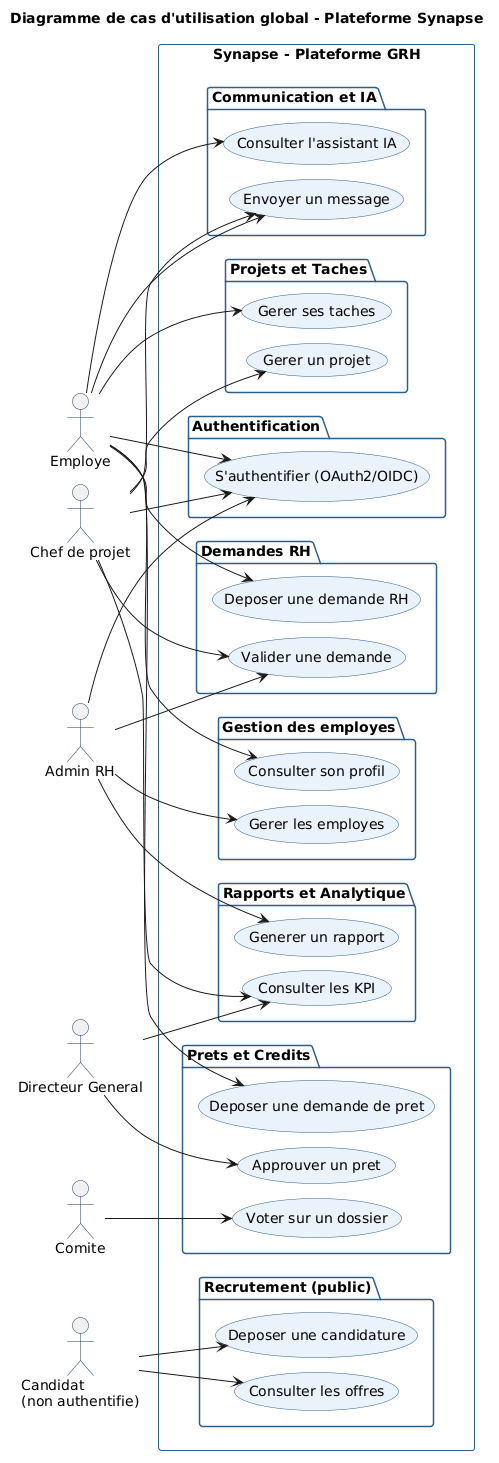
\includegraphics[width=0.78\textwidth,height=0.50\textheight,keepaspectratio]{diagrams/uc_global_synapse.png}
  \caption{Diagramme de cas d’utilisation global de Synapse}
  \label{fig:usecase_global}
\end{figure}

\subsection{Cas d’utilisation~: Gestion des demandes RH}

\begin{figure}[H]
\centering
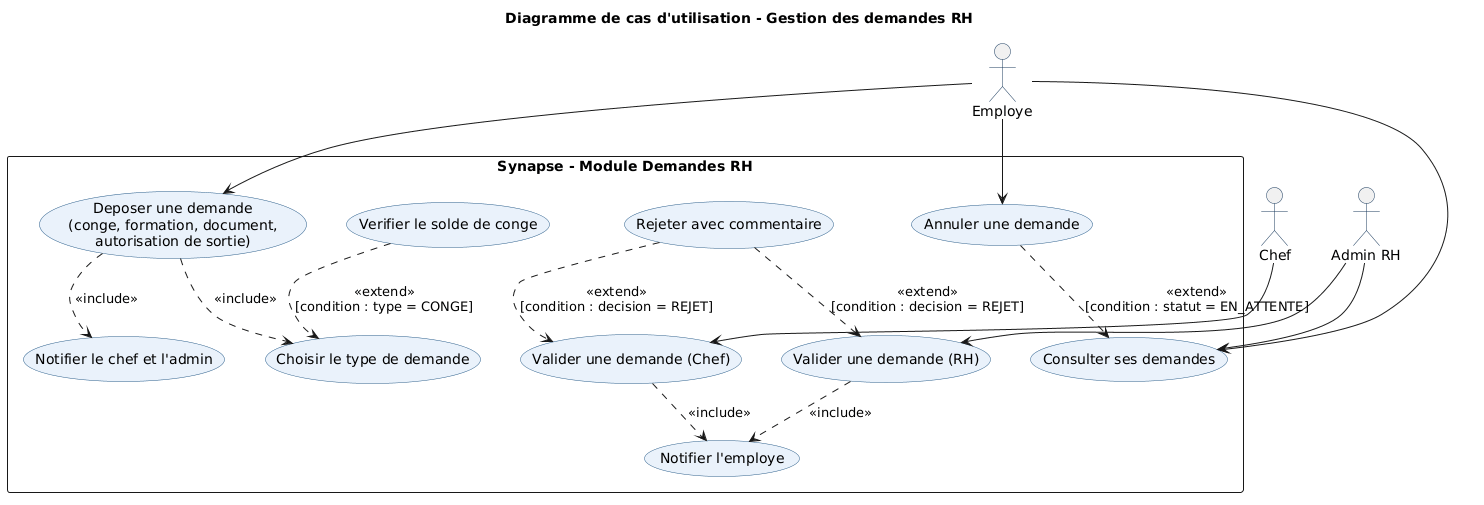
\includegraphics[width=0.90\textwidth,height=0.58\textheight,keepaspectratio]{diagrams/uc_depot_validation_demande_rh.png}
\caption{Diagramme de cas d’utilisation~: gestion des demandes RH}
\label{fig:usecase_demandes}
\end{figure}

\subsection{Cas d’utilisation~: Gestion des employés}

\begin{figure}[H]
  \centering
  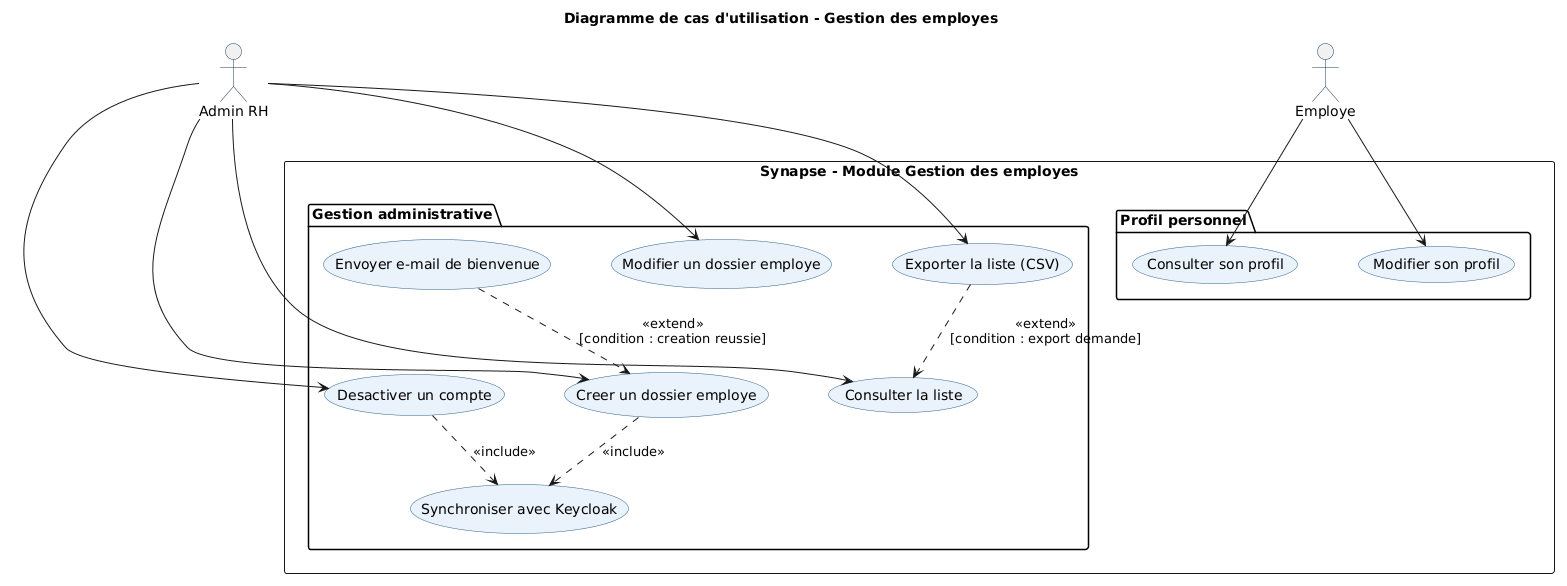
\includegraphics[width=0.90\textwidth,height=0.58\textheight,keepaspectratio]{diagrams/uc_gerer_employes.png}
  \caption{Diagramme de cas d’utilisation~: gestion des employés}
  \label{fig:usecase_employes}
\end{figure}

\subsection{Cas d’utilisation~: Gestion des projets et tâches}

\begin{figure}[H]
  \centering
  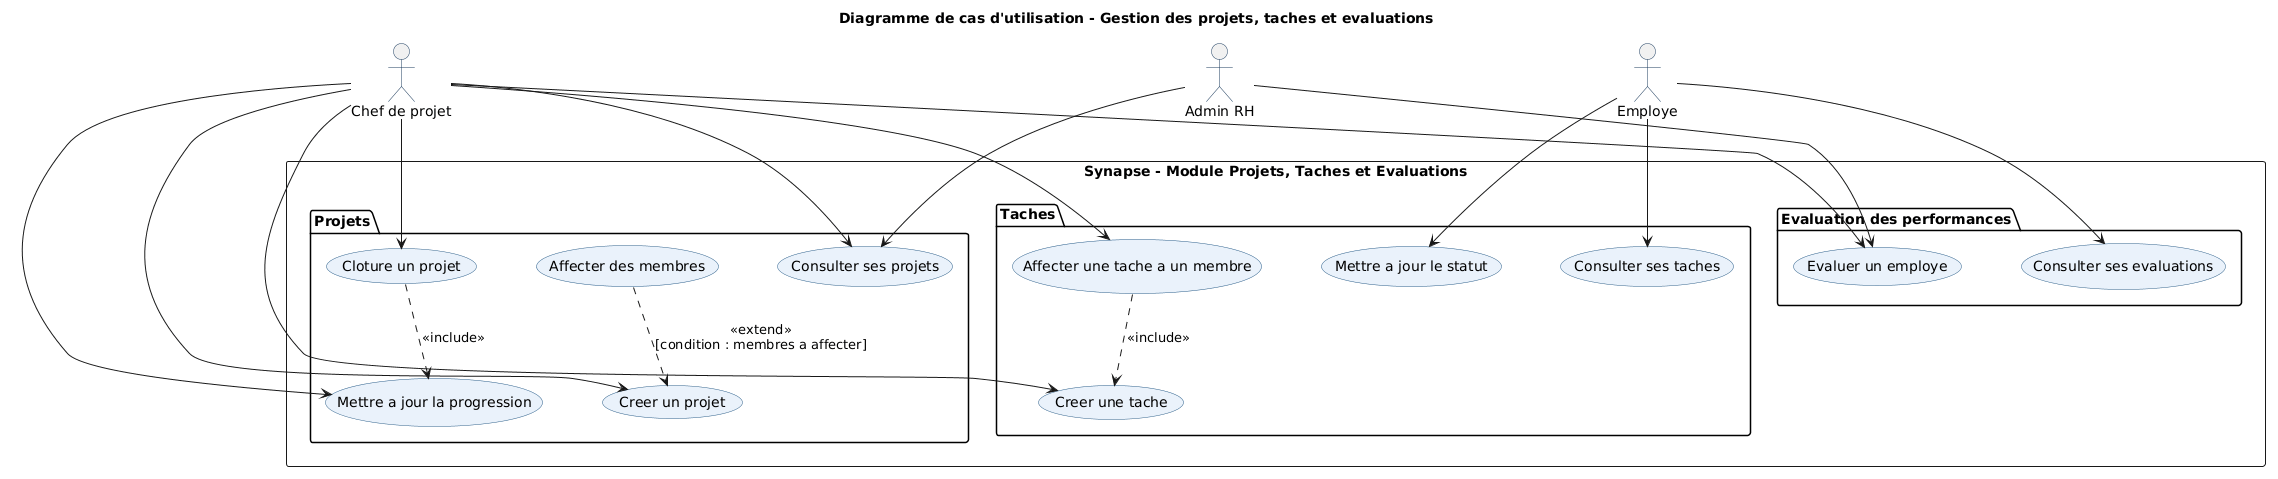
\includegraphics[width=0.90\textwidth,height=0.58\textheight,keepaspectratio]{diagrams/uc_projets_taches_chef.png}
  \caption{Diagramme de cas d’utilisation~: gestion des projets et tâches}
  \label{fig:usecase_projets}
\end{figure}

\section{Architecture générale de Synapse}

Synapse repose sur une architecture microservices composée de sept services Spring Boot
indépendants, chacun dédié à un domaine fonctionnel précis~: \textit{employe-service},
\textit{demandes-service}, \textit{chat-service}, \textit{notification-service},
\textit{projets-service}, \textit{taches-service} et \textit{analytics-service}.
Tous sont sécurisés par un serveur Keycloak centralisé via le protocole OAuth2/OIDC,
communiquent de manière asynchrone via Apache Kafka pour les notifications,
et sont conteneurisés sous Docker Compose pour garantir la reproductibilité
de l'environnement.

\begin{figure}[H]
\centering
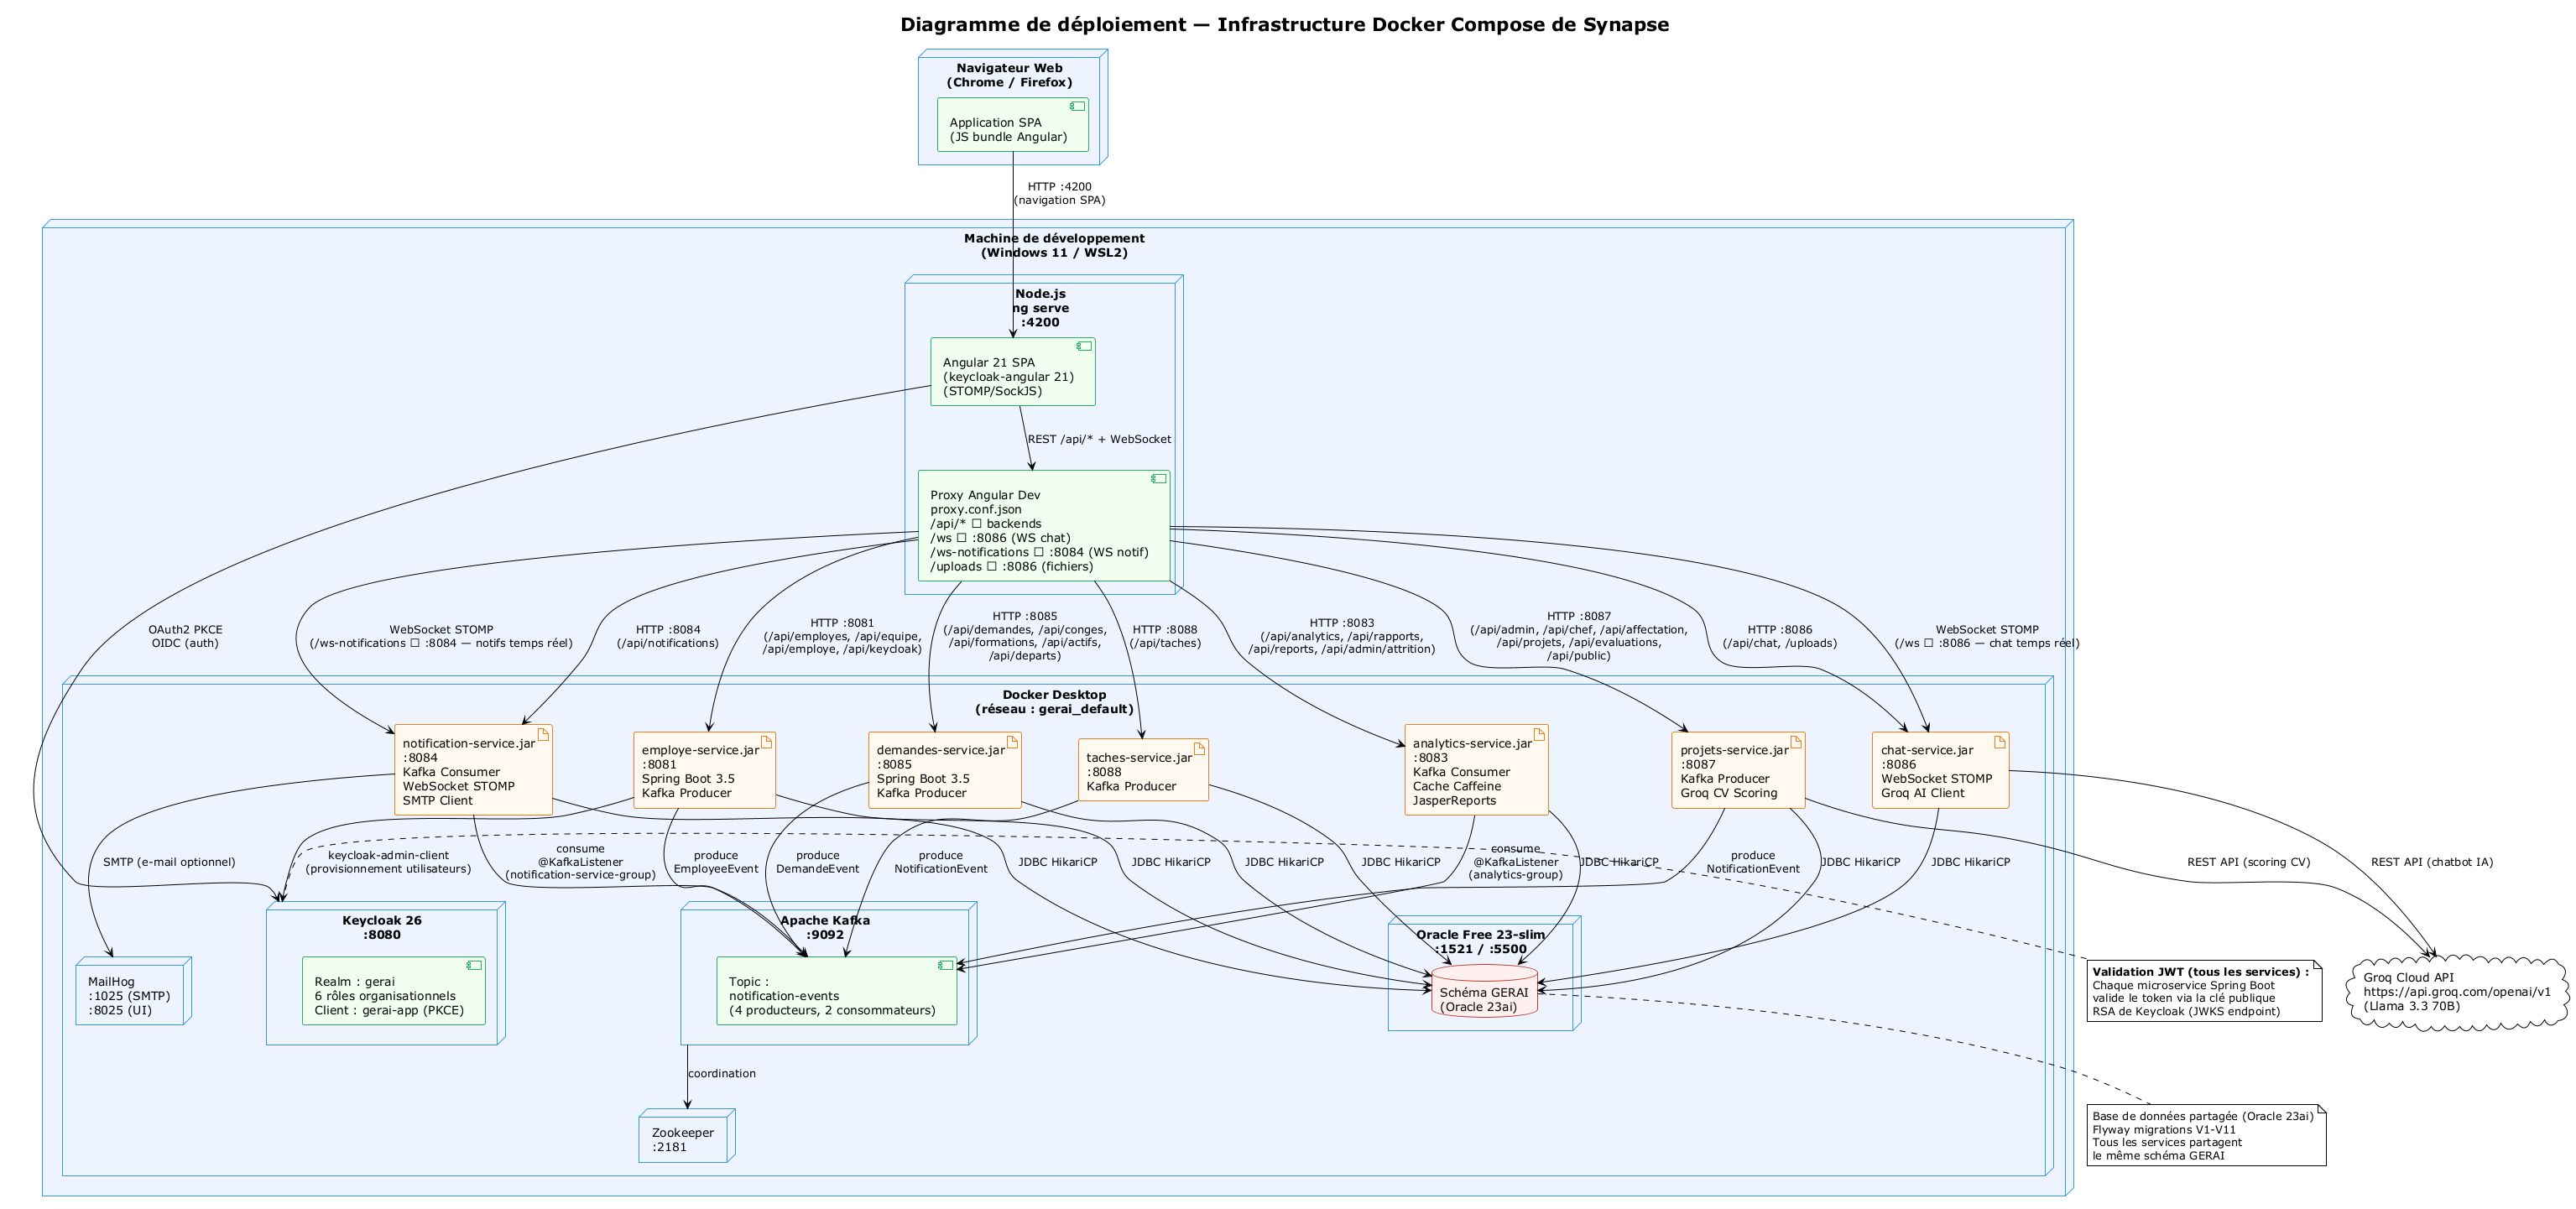
\includegraphics[width=0.88\textwidth,height=0.52\textheight,keepaspectratio]{images/deployment_docker.png}
\caption{Diagramme de déploiement~: architecture microservices et conteneurs Docker Compose}
\label{fig:deployment}
\end{figure}

Le frontend Angular~21 consomme les API REST de chaque service via un Bearer token JWT.
La base de données Oracle~23ai est partagée entre les services via un schéma unique
(\texttt{GERAI}), versionné par Flyway. Les échanges synchrones utilisent HTTP/REST~; les échanges
asynchrones transitent par des topics Kafka.

\section{Modélisation des données}

\subsection{Diagramme de classes principal}

Le diagramme de classes de la figure~\ref{fig:class_diagram} représente les entités
métier principales de Synapse et leurs associations. L'entité \texttt{Employee} est
centrale~: elle est référencée par \texttt{Demande}, \texttt{Projet}, \texttt{Message}
et \texttt{AttritionPrediction}. Chaque \texttt{Demande} possède un statut évoluant
au fil du workflow de validation~; chaque \texttt{Projet} agrège des \texttt{Tache}
dont les statuts déterminent le calcul automatique de la progression.

\begin{figure}[H]
  \centering
  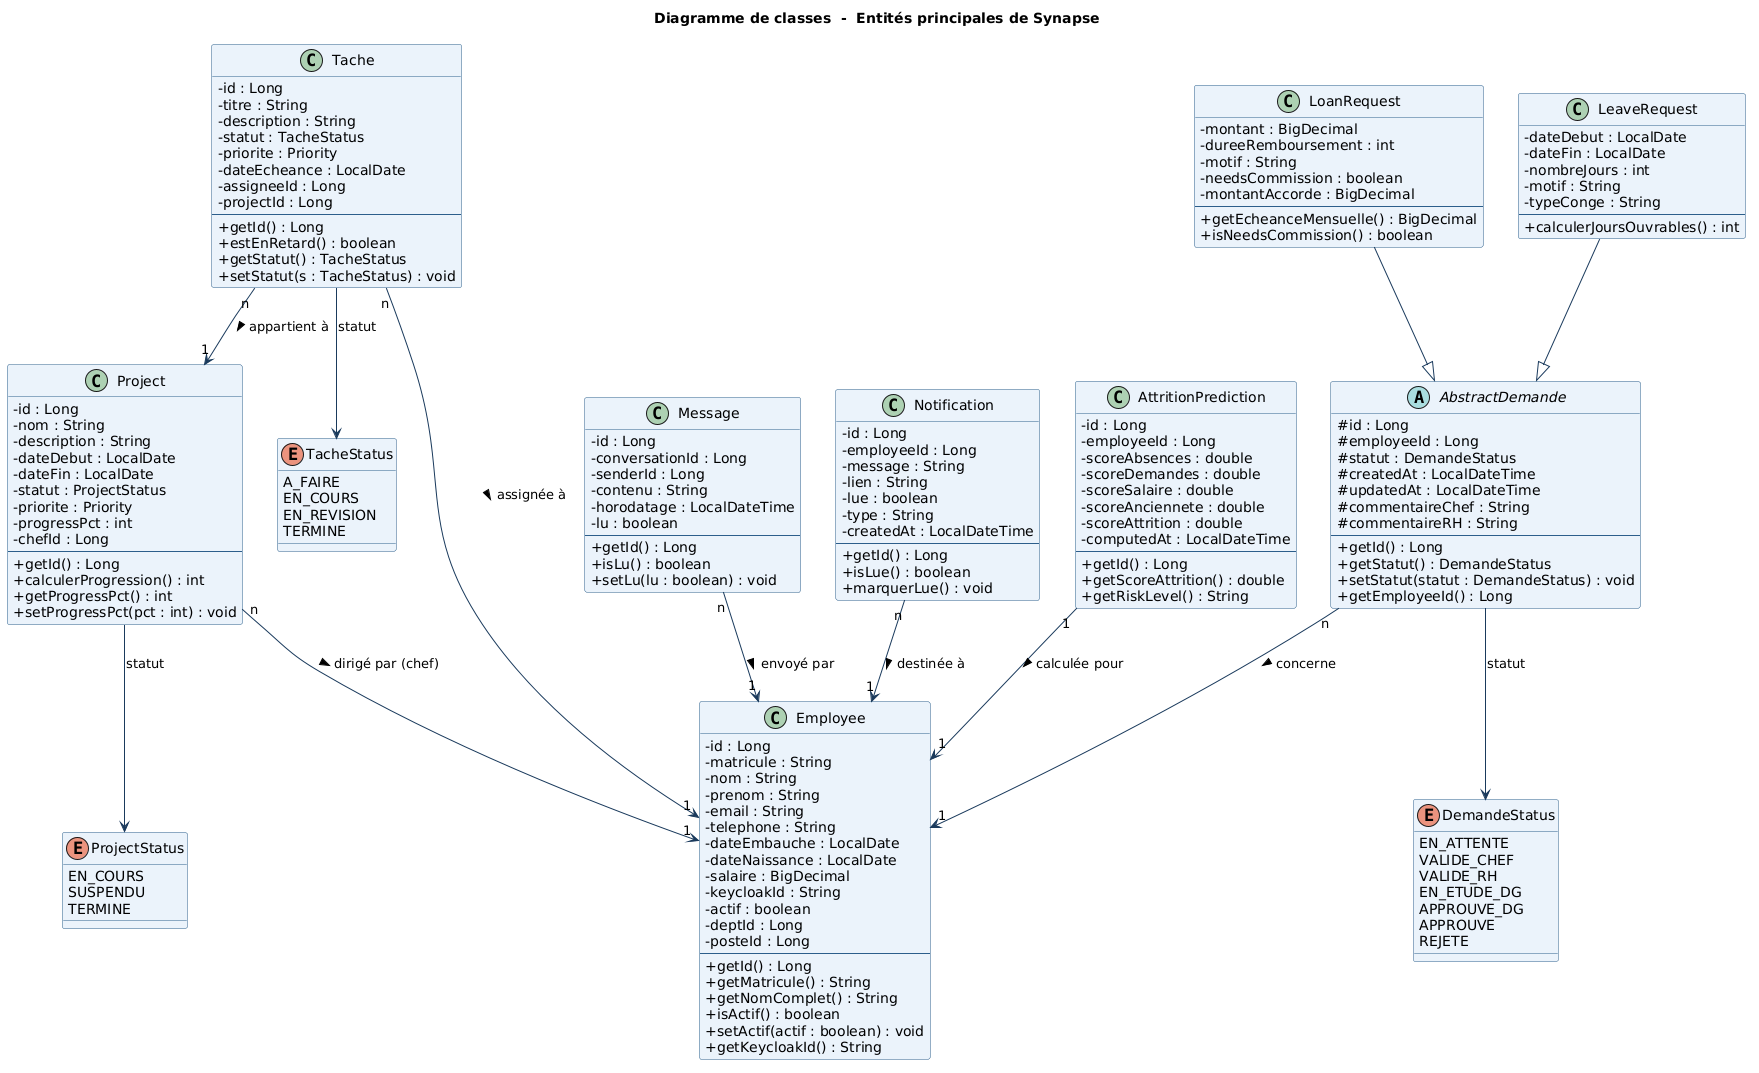
\includegraphics[width=\textwidth,height=0.58\textheight,keepaspectratio]{diagrams/class_diagram_principal.png}
  \caption{Diagramme de classes des entités principales de Synapse}
  \label{fig:class_diagram}
\end{figure}

\subsection{Schéma de base de données (extrait)}

Le schéma entité-association de la figure~\ref{fig:schema_er} présente les tables
Oracle~23ai correspondant aux domaines RH et projets. La table \texttt{EMPLOYEES}
constitue la clé étrangère de référence pour \texttt{LEAVE\_REQUESTS},
\texttt{PROJECTS} et \texttt{TASKS}. Les contraintes d'intégrité et les migrations sont gérées par Flyway~; onze scripts
de migration (V1 à V11) ont été exécutés au démarrage pour initialiser le schéma
complet. Le tableau~\ref{tab:flyway_map} résume l'affectation de chaque migration
à son domaine fonctionnel.

\begin{table}[H]
\centering
\caption{Affectation des migrations Flyway aux domaines fonctionnels}
\label{tab:flyway_map}
\begin{tabularx}{\textwidth}{VlVlVLV}
\rowcolor{headerblue!55}
\hline
\textbf{Migration} & \textbf{Sprint} & \textbf{Domaine} \\
\hline
V1 & 1 & Core RH~: \texttt{EMPLOYEES}, \texttt{DEPARTMENTS}, \texttt{POSITIONS}, \texttt{CONTRACTS} \\
\hline
V2 & 1 (schéma) / 6 (implem.) & Projets, tâches, évaluations de performances \\
\hline
V3 & 1 (schéma) / 3 (implem.) & Demandes RH~: congés, prêts, formations, autorisations, documents \\
\hline
V4 & 1 (schéma) / 4-5 (implem.) & Communication~: conversations, messages, notifications \\
\hline
V5 & Hors scope & Présence et paie~: tables \texttt{ATTENDANCE}, \texttt{PAYSLIPS} (schéma défini pour extension future~; module non implémenté dans le périmètre du projet) \\
\hline
V6 & 7 & Reporting, audit (\texttt{AUDIT\_LOGS}) et prédictions ML \\
\hline
V7--V9 & 1 & Données de référence et jeux de démonstration \\
\hline
V10 & 7 & Vue analytique \texttt{V\_ALL\_DEMANDES} \\
\hline
V11 & 2 & Colonne \texttt{employee\_code} (\texttt{EMP-XXXX}) \\
\hline
\end{tabularx}
\end{table}

\begin{figure}[H]
  \centering
  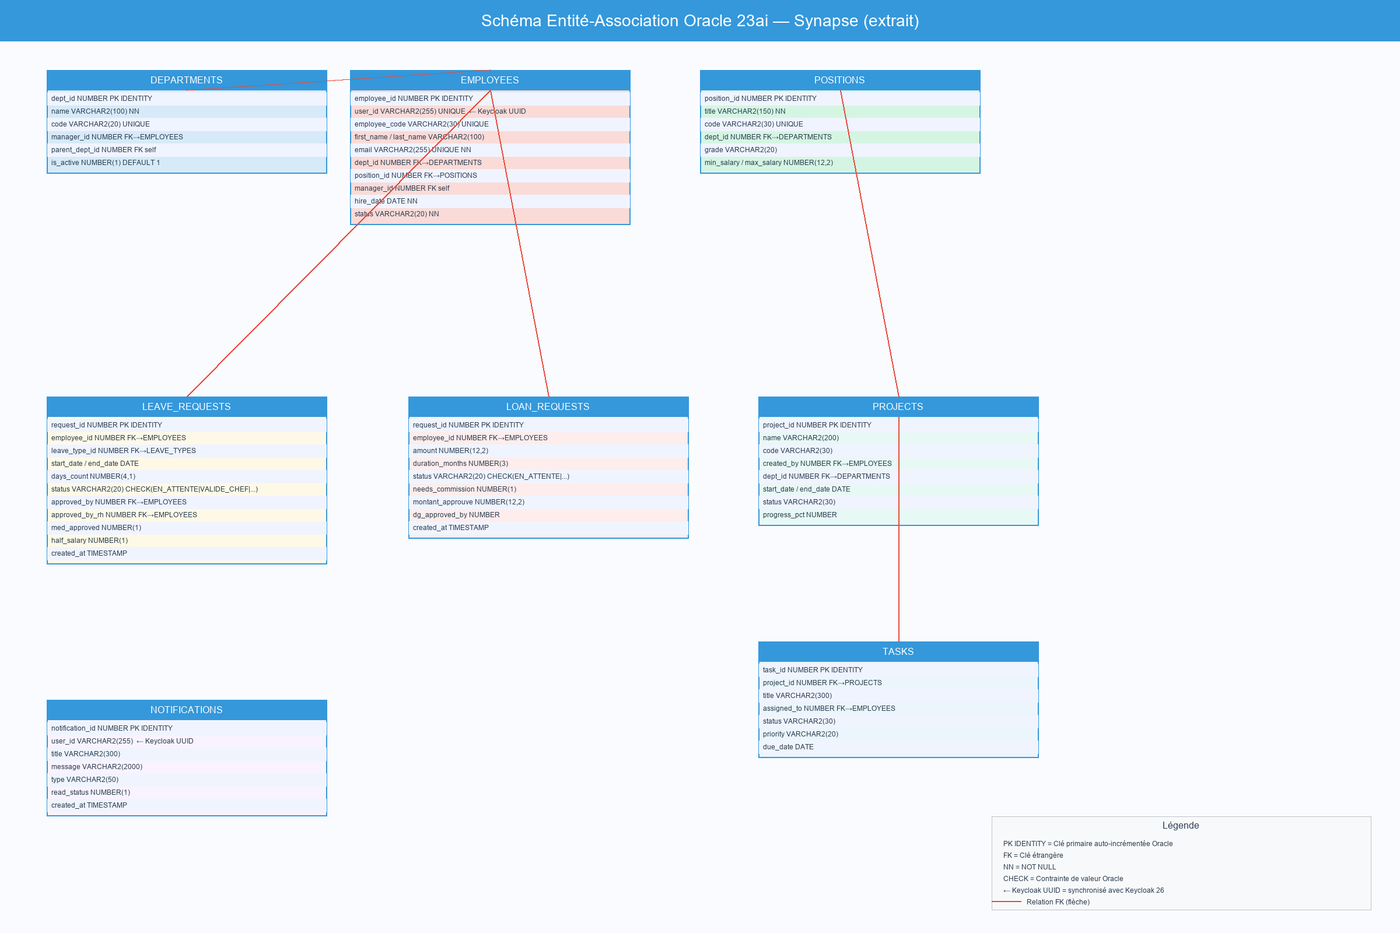
\includegraphics[width=0.88\textwidth,height=0.52\textheight,keepaspectratio]{images/schema_er_oracle.png}
  \caption{Schéma entité-association Oracle 23ai (extrait~: tables RH et projets)}
  \label{fig:schema_er}
\end{figure}

% ─────────────────────────────────────────────────────────────
\section{Environnement de développement}
% ─────────────────────────────────────────────────────────────

\subsection{Environnement matériel}

La table~\ref{tab:hardware} ci-dessous présente les postes de travail utilisés pour
le développement du projet.

\begin{table}[H]
\centering
\caption{Environnement matériel}
\label{tab:hardware}
\begin{tabularx}{\textwidth}{VlVXVXV}
\rowcolor{headerblue!55}
\hline
\textbf{Composant} & \textbf{Poste 1} & \textbf{Poste 2} \\
\hline
Processeur & Intel Core i5-1235U (12\textsuperscript{e} génération), 1,30~GHz, 10 cœurs & Intel Core i7-13700H (13\textsuperscript{e} génération), 2,4~GHz \\
\hline
RAM & 20 Go & 32 Go DDR4 \\
\hline
Système d’exploitation & Windows 11 Professionnel 64 bits & Windows 11 Professionnel 64 bits \\
\hline
Stockage & SSD 512 Go & SSD 1 To (Samsung NVMe) \\
\hline
\end{tabularx}
\end{table}

\subsection{Logiciels et environnements de développement}

Le tableau~\ref{tab:tools_ides} présente les environnements de développement intégrés
utilisés pour le codage, le débogage et l'exécution du projet.

\begin{table}[H]
\centering
\caption{Environnements de développement intégrés}
\label{tab:tools_ides}
\begin{tabularx}{\textwidth}{V>{\centering\arraybackslash}m{3.2cm}|X|}
\rowcolor{headerblue!55}
\hline
\textbf{Logo} & \textbf{Description} \\
\hline
\centering
\includegraphics[height=1.4cm,keepaspectratio]{images/logo_intellij.png} &
IntelliJ IDEA\textsuperscript{[20]}, IDE retenu pour le développement backend de Synapse grâce à sa
prise en charge native de Spring Boot, Maven et JPA~; il a servi à écrire,
déboguer et tester les sept microservices Java tout au long des sept sprints \\
\hline
\centering
\includegraphics[height=1.4cm,keepaspectratio]{images/logo_vscode.png} &
Visual Studio Code\textsuperscript{[21]}, choisi pour le développement du frontend Angular~21 de
Synapse~; les extensions Angular Language Service, ESLint et Prettier ont
été configurées pour garantir la cohérence du code TypeScript entre les
composants standalone \\
\hline
\end{tabularx}
\end{table}

Le tableau~\ref{tab:tools_tests} présente les outils de test et de validation des API
utilisés pour vérifier le bon fonctionnement des endpoints REST.

\begin{table}[H]
\centering
\caption{Outils de test et validation d'API}
\label{tab:tools_tests}
\begin{tabularx}{\textwidth}{V>{\centering\arraybackslash}m{3.2cm}|X|}
\rowcolor{headerblue!55}
\hline
\textbf{Logo} & \textbf{Description} \\
\hline
\centering
\includegraphics[height=1.4cm,keepaspectratio]{images/logo_postman.png} &
Postman\textsuperscript{[22]}, utilisé pour valider les douze endpoints critiques de Synapse~;
chaque requête de la collection porte un Bearer token JWT émis par Keycloak,
ce qui permet de vérifier simultanément la logique métier et l'application
des règles RBAC sur chaque microservice \\
\hline
\end{tabularx}
\end{table}

Le tableau~\ref{tab:tools_devops} présente les outils de conteneurisation et
d'infrastructure utilisés pour reproduire l'environnement d'exécution de Synapse.

\begin{table}[H]
\centering
\caption{Conteneurisation et infrastructure}
\label{tab:tools_devops}
\begin{tabularx}{\textwidth}{V>{\centering\arraybackslash}m{3.2cm}|X|}
\rowcolor{headerblue!55}
\hline
\textbf{Logo} & \textbf{Description} \\
\hline
\centering
\includegraphics[height=1.4cm,keepaspectratio]{images/logo_docker.png} &
Docker Desktop, moteur de conteneurisation retenu pour isoler et reproduire
l'infrastructure locale de Synapse~: Oracle~23ai, Keycloak~26, Apache Kafka,
Zookeeper et MailHog sont démarrés en une seule commande
\texttt{docker-compose up}, garantissant un environnement identique sur toute
machine de développement \\
\hline
\end{tabularx}
\end{table}

Le tableau~\ref{tab:tools_bdd} présente l'outil d'administration de base de données
utilisé pour inspecter et requêter le schéma Oracle~23ai.

\begin{table}[H]
\centering
\caption{Administration de base de données}
\label{tab:tools_bdd}
\begin{tabularx}{\textwidth}{V>{\centering\arraybackslash}m{3.2cm}|X|}
\rowcolor{headerblue!55}
\hline
\textbf{Logo} & \textbf{Description} \\
\hline
\centering
\includegraphics[height=1.4cm,keepaspectratio]{images/logo_dbeaver.png} &
DBeaver\textsuperscript{[28]}, client universel de base de données open source permettant
l'administration, l'inspection et l'exécution de requêtes SQL directement
sur la base Oracle~23ai de Synapse \\
\hline
\end{tabularx}
\end{table}

Le tableau~\ref{tab:tools_conception} présente les outils de modélisation utilisés
pour produire les diagrammes UML du rapport.

\begin{table}[H]
\centering
\caption{Conception et modélisation UML}
\label{tab:tools_conception}
\begin{tabularx}{\textwidth}{V>{\centering\arraybackslash}m{3.2cm}|X|}
\rowcolor{headerblue!55}
\hline
\textbf{Logo} & \textbf{Description} \\
\hline
\centering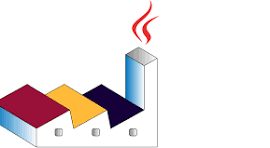
\includegraphics[height=1.4cm,keepaspectratio]{images/logo_plantuml.png} &
PlantUML\textsuperscript{[29]}, outil de génération de diagrammes UML à partir de fichiers source
\texttt{.puml} versionnés~; les diagrammes de cas d'utilisation, séquence,
déploiement et classes ont été générés dans le répertoire
\texttt{docs/plantuml/} \\
\hline

\includegraphics[height=1.4cm,keepaspectratio]{images/logo_drawio.png} &
draw.io\textsuperscript{[23]}, outil de diagrammatique en ligne utilisé pour la conception
des maquettes d'architecture et des schémas de flux~; les fichiers \texttt{.drawio}
ont servi de support de travail collaboratif avant exportation vers les formats
définitifs intégrés au rapport \\
\hline
\end{tabularx}
\end{table}

Le tableau~\ref{tab:tools_gestion} présente l'outil de gestion de version utilisé
tout au long du projet.

\begin{table}[H]
\centering
\caption{Gestion de version}
\label{tab:tools_gestion}
\begin{tabularx}{\textwidth}{V>{\centering\arraybackslash}m{3.2cm}|X|}
\rowcolor{headerblue!55}
\hline
\textbf{Logo} & \textbf{Description} \\
\hline
\centering
\includegraphics[height=1.4cm,keepaspectratio]{images/logo_github.png} &
GitHub\textsuperscript{[24]}, dépôt distant hébergeant les deux dépôts du projet Synapse
(frontend Angular et backend Spring Boot)~; le workflow de branches
(\texttt{feature} $\rightarrow$ \texttt{develop} $\rightarrow$ \texttt{main})
a structuré le développement sprint par sprint et assuré la traçabilité
des livraisons jusqu'à la version finale \\
\hline
\end{tabularx}
\end{table}

Le tableau~\ref{tab:tools_qualite} présente l'outil de mesure de couverture de tests
intégré aux builds Maven de Synapse.

\begin{table}[H]
\centering
\caption{Mesure de couverture de tests}
\label{tab:tools_qualite}
\begin{tabularx}{\textwidth}{V>{\centering\arraybackslash}m{3.2cm}|X|}
\rowcolor{headerblue!55}
\hline
\textbf{Logo} & \textbf{Description} \\
\hline
\centering
\includegraphics[height=1.4cm,keepaspectratio]{images/logo_jacoco.png} &
JaCoCo\textsuperscript{[30]} (Java Code Coverage), plugin Maven qui mesure la couverture d'instructions
et de branches lors de l'exécution de la suite de tests~; intégré à
l'\textit{analytics-service} et au \textit{projets-service} avec un seuil
minimal de 50\,\% configuré dans \texttt{pom.xml} \\
\hline
\end{tabularx}
\end{table}

% ─────────────────────────────────────────────────────────────
\section{Planification du projet}
% ─────────────────────────────────────────────────────────────

\subsection{Équipe Scrum et rôles}

La table~\ref{tab:scrum_team} ci-dessous présente l'équipe Scrum et les rôles
associés.

\begin{table}[H]
\centering
\caption{Équipe Scrum et rôles}
\label{tab:scrum_team}
\begin{tabularx}{\textwidth}{VlVlVLV}
\rowcolor{headerblue!55}
\hline
\textbf{Rôle} & \textbf{Acteur} & \textbf{Mission} \\
\hline
Product Owner & Mouadh Zidi & Définir et prioriser le backlog selon les besoins d'Arabsoft \\
\hline
Scrum Master & Sofiene Melki & Faciliter les cérémonies Scrum et lever les obstacles \\
\hline
Équipe de développement & Mariem Saadaoui \& Nour Elhouda Boussaidi & Concevoir, développer, tester et livrer la solution \\
\hline
\end{tabularx}
\end{table}

\subsection{Planification des sprints}

La table~\ref{tab:sprint_plan} présente la répartition des sprints par release
avec leurs dates réelles de réalisation (projet débuté le 2~février~2026).

\begin{table}[H]
\centering
\caption{Planification des sprints par release et période}
\label{tab:sprint_plan}
\begin{tabularx}{\textwidth}{VCVlVLVlV}
\rowcolor{headerblue!55}
\hline
\textbf{Release} & \textbf{Sprint} & \textbf{Contenu principal} & \textbf{Période} \\
\hline
\multirow{2}{*}{Release 1} & Sprint 1 & Infrastructure, Keycloak, Oracle, Angular & 02--15 fév. 2026 \\
\hline
& Sprint 2 & employe-service, sync Oracle--Keycloak, matricules & 16 fév.--01 mars 2026 \\
\hline
\multirow{3}{*}{Release 2} & Sprint 3 & Demandes RH (congés, formations, documents) & 02--15 mars 2026 \\
\hline
& Sprint 4 & Prêts/crédits, circuit DG/comité, Kafka & 16--29 mars 2026 \\
\hline
& Sprint 5 & Chat WebSocket, assistant IA Groq & 30 mars--12 avr. 2026 \\
\hline
\multirow{2}{*}{Release 3} & Sprint 6 & Projets, tâches, évaluation, recrutement IA & 13--26 avr. 2026 \\
\hline
& Sprint 7 & JasperReports, analytics, prédiction attrition & 27 avr.--10 mai 2026 \\
\hline
\end{tabularx}
\end{table}

% Insert figure: Feuille de route du projet (Gantt ou roadmap visuelle)
\begin{figure}[H]
  \centering
  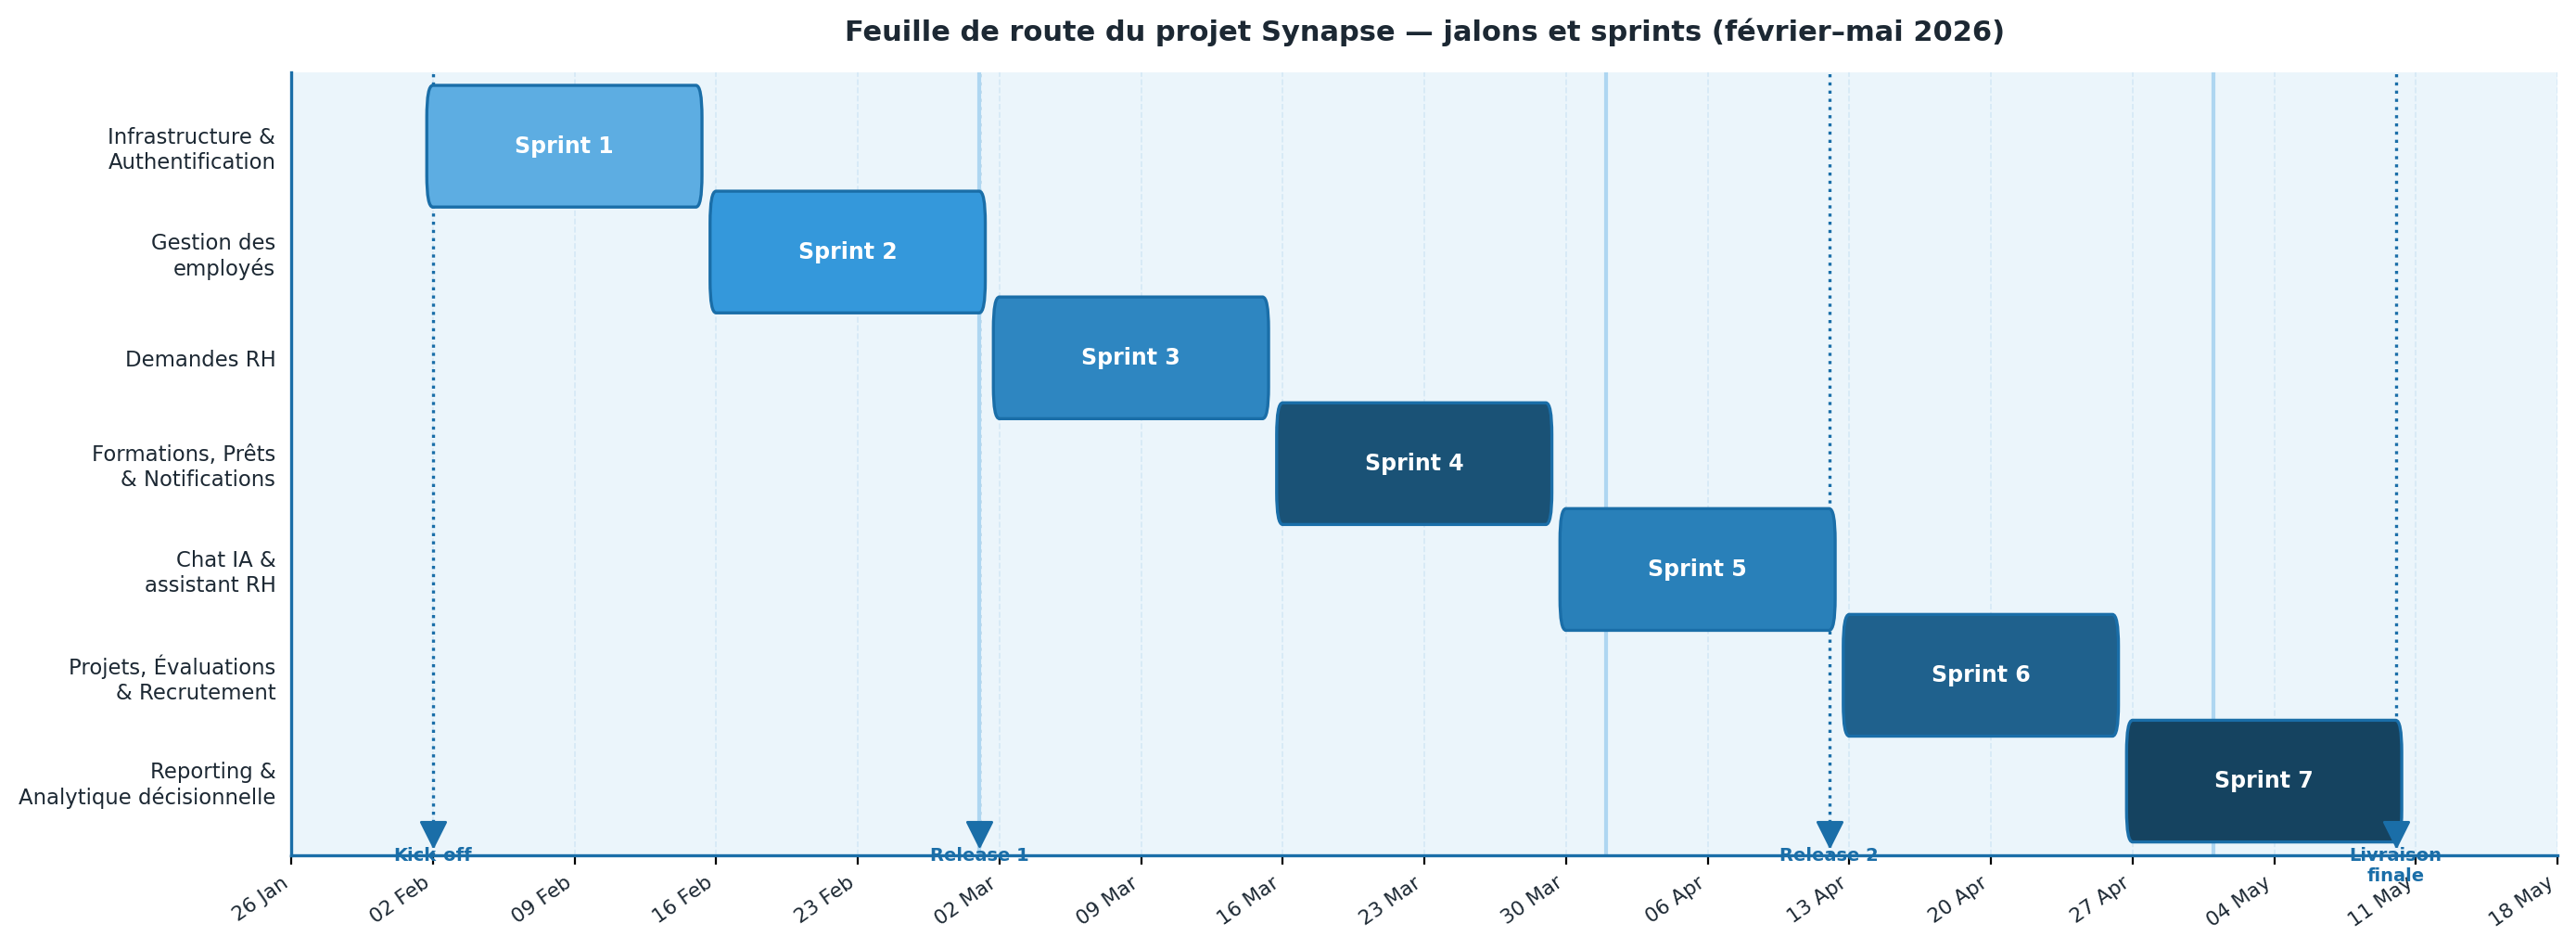
\includegraphics[width=0.88\textwidth,height=0.52\textheight,keepaspectratio]{images/roadmap_projet.png}
  \caption{Feuille de route du projet Synapse~: jalons et sprints (février--mai~2026)}
  \label{fig:roadmap}
\end{figure}

% ─────────────────────────────────────────────────────────────
% !TEX root = ./rapport.tex
% ══════════════════════════════════════════════════════════════════════
%  ÉTUDE ET JUSTIFICATION DES CHOIX TECHNOLOGIQUES
%  Inclure dans chapitre 2 via : % !TEX root = ./rapport.tex
% ══════════════════════════════════════════════════════════════════════
%  ÉTUDE ET JUSTIFICATION DES CHOIX TECHNOLOGIQUES
%  Inclure dans chapitre 2 via : % !TEX root = ./rapport.tex
% ══════════════════════════════════════════════════════════════════════
%  ÉTUDE ET JUSTIFICATION DES CHOIX TECHNOLOGIQUES
%  Inclure dans chapitre 2 via : \input{choix_technologiques}
% ══════════════════════════════════════════════════════════════════════

\section{Étude et justification des choix technologiques}

Chaque décision technologique de Synapse est documentée en deux temps~:
d'abord la justification de la \textbf{catégorie} de technologie retenue
(pourquoi ce type d'outil est nécessaire, et quelle alternative naïve a été
écartée et pourquoi), puis la justification du \textbf{produit spécifique}
choisi au sein de cette catégorie, étayée par une comparaison explicite
d'alternatives sur des critères mesurables.

% ──────────────────────────────────────────────────────────────────────
\subsection{Architecture applicative~: microservices vs monolithique}
% ──────────────────────────────────────────────────────────────────────

\subsubsection*{Pourquoi cette catégorie~?}

Synapse couvre sept domaines fonctionnels aux exigences hétérogènes~: l'\textit{analytics-service} est intensif en I/O de lecture, le \textit{chat-service} maintient des connexions WebSocket persistantes, les demandes RH publient des événements Kafka asynchrones. Regrouper ces domaines dans un seul déployable forcerait un couplage structurel rendant tout déploiement partiel impossible et toute modification d'un module risquée pour l'ensemble de l'application.

\subsubsection*{Présentation}

L'\textbf{architecture microservices} décompose une application en services
autonomes, faiblement couplés, chacun exposant une API REST, gérant sa propre
logique métier et déployable indépendamment. L'\textbf{architecture monolithique}
regroupe l'ensemble des fonctionnalités dans un seul déployable, tandis que
l'\textbf{architecture orientée services (SOA)} propose un découpage plus grossier
reposant sur un bus d'intégration (ESB).

\subsubsection*{Comparaison}

\begin{table}[H]
\centering
\caption{Comparaison des styles architecturaux}
\label{tab:cmp_architecture}
\begin{tabularx}{\textwidth}{VlVCVCVCV}
\rowcolor{headerblue!55}
\hline
\textbf{Critère} & \textbf{Monolithique} & \textbf{SOA} & \textbf{Microservices} \\
\hline
Scalabilité indépendante     & Faible   & Moyen    & \textbf{Excellent} \\
\hline
Isolation des pannes         & Faible   & Moyen    & \textbf{Excellent} \\
\hline
Déploiement indépendant      & Non      & Partiel  & \textbf{Oui} \\
\hline
Hétérogénéité technologique  & Non      & Partiel  & \textbf{Oui} \\
\hline
Complexité opérationnelle    & \textbf{Faible} & Moyenne & Élevée \\
\hline
Adapté à un domaine découpé  & Moyen    & Bon      & \textbf{Excellent} \\
\hline
\end{tabularx}
\end{table}

\subsubsection*{Justification du choix}

Les sept domaines de Synapse ont des exigences incompatibles dans un seul déployable~: l'\textit{analytics-service} est intensif en I/O, le \textit{chat-service} maintient des connexions persistantes. L'architecture microservices permet de scaler et de faire évoluer chaque service indépendamment, et garantit que la défaillance d'un service n'affecte pas les autres.

% ──────────────────────────────────────────────────────────────────────
\subsection{Framework frontend~: Angular 21}
% ──────────────────────────────────────────────────────────────────────

\subsubsection*{Pourquoi cette catégorie~?}

Les notifications temps réel et les mises à jour de tableaux de bord sans rechargement sont structurellement incompatibles avec un rendu côté serveur (Thymeleaf, JSP)~: chaque action impliquerait un rechargement complet de la page. Une \textbf{Single-Page Application} (SPA) maintient l'état en mémoire et communique avec le backend via API REST et WebSocket, ce qui est indispensable pour la messagerie instantanée et le push de notifications de Synapse.

\subsubsection*{Présentation}

\textbf{Angular}\textsuperscript{[4]} est un framework SPA de Google basé sur TypeScript. Il impose
une architecture MVC stricte avec injection de dépendances intégrée, un système de
composants standalone (depuis Angular~14), un compilateur Ivy et des outils de
routage, de formulaires réactifs et d'intercepteurs HTTP inclus nativement.

\subsubsection*{Comparaison}

\begin{table}[H]
\centering
\caption{Comparaison des frameworks SPA frontend}
\label{tab:cmp_frontend}
\begin{tabularx}{\textwidth}{VlVCVCVCV}
\rowcolor{headerblue!55}
\hline
\textbf{Critère} & \textbf{React 18} & \textbf{Vue 3} & \textbf{Angular 21} \\
\hline
Typage TypeScript natif       & Partiel  & Partiel  & \textbf{Natif} \\
\hline
Architecture structurée       & Libre    & Libre    & \textbf{Imposée} \\
\hline
Intégration Keycloak officielle & Communauté & Communauté & \textbf{keycloak-angular} \\
\hline
Injection de dépendances      & Externe  & Externe  & \textbf{Intégrée} \\
\hline
Guards de routage             & Manuel   & Manuel   & \textbf{Natif} \\
\hline
Adapté aux SPA multi-rôles   & Moyen    & Moyen    & \textbf{Excellent} \\
\hline
Courbe d'apprentissage        & \textbf{Faible} & \textbf{Faible} & Élevée \\
\hline
\end{tabularx}
\end{table}

\subsubsection*{Avantages et inconvénients}

\begin{itemize}[leftmargin=*,nosep]
  \item \textbf{Avantages}~: architecture opinionated adaptée aux grandes équipes,
        bibliothèque \texttt{keycloak-angular} officielle, guards de routage natifs
        pour le RBAC, détection de changement OnPush pour les tableaux de bord, lazy
        loading des modules par rôle.
  \item \textbf{Inconvénients}~: courbe d'apprentissage plus élevée que React/Vue,
        bundle initial plus lourd sans tree-shaking agressif.
\end{itemize}

\subsubsection*{Justification du choix}

Le RBAC multi-rôles de Synapse est implémenté en un \texttt{requireRoleGuard} réutilisable sur chaque route, grâce à l'intégration native \texttt{keycloak-angular}. Les intercepteurs HTTP centralisent l'injection du Bearer token pour tous les services, et la stratégie \texttt{OnPush} des composants de tableaux de bord évite les rendus inutiles sans gestionnaire d'état externe.

% ──────────────────────────────────────────────────────────────────────
\subsection{Framework backend~: Spring Boot 3.5}
% ──────────────────────────────────────────────────────────────────────

\subsubsection*{Pourquoi cette catégorie~?}

Les sept microservices doivent exposer des API REST, valider des tokens JWT, persister en Oracle, publier des événements Kafka et, pour certains, envoyer des e-mails ou maintenir des connexions WebSocket. Sans framework, chaque service devrait implémenter manuellement le serveur HTTP, la désérialisation JSON, la gestion des transactions et le pool de connexions~; un \textbf{framework de microservices} industrialise ces préoccupations transversales et garantit la cohérence de configuration sur l'ensemble des services.

\subsubsection*{Présentation}

\textbf{Spring Boot}\textsuperscript{[6]} est un framework Java/JVM qui simplifie la création de
microservices REST via une auto-configuration et un serveur embarqué Tomcat. Il
fédère l'écosystème Spring~: Security, Data JPA, Kafka, Mail, Cache, Validation,
WebSocket.

\subsubsection*{Comparaison}

\begin{table}[H]
\centering
\caption{Comparaison des frameworks backend Java}
\label{tab:cmp_backend}
\begin{tabularx}{\textwidth}{VlVCVCVCV}
\rowcolor{headerblue!55}
\hline
\textbf{Critère} & \textbf{Node.js/Express} & \textbf{Quarkus} & \textbf{Spring Boot 3.5} \\
\hline
Écosystème JVM/Java          & N/A      & Excellent & \textbf{Excellent} \\
\hline
Intégration Keycloak OAuth2  & Externe  & Bon       & \textbf{Natif (starter)} \\
\hline
Support JPA + Oracle OJDBC   & Non      & Bon       & \textbf{Excellent} \\
\hline
spring-kafka natif           & Non      & Bon       & \textbf{Natif} \\
\hline
Temps de démarrage           & Très rapide & Très rapide & Moyen \\
\hline
Maturité / documentation     & Excellente & Moyenne  & \textbf{Très élevée} \\
\hline
\end{tabularx}
\end{table}

\subsubsection*{Avantages et inconvénients}

\begin{itemize}[leftmargin=*,nosep]
  \item \textbf{Avantages}~: couverture fonctionnelle complète en un seul écosystème
        (sécurité, persistance, messaging, cache, email), annotation
        \texttt{@PreAuthorize} pour le RBAC déclaratif, starter
        \texttt{oauth2-resource-server} pour la validation JWT Keycloak.
  \item \textbf{Inconvénients}~: temps de démarrage plus long que Quarkus en mode
        JVM, empreinte mémoire plus élevée.
\end{itemize}

\subsubsection*{Justification du choix}

Chaque microservice utilise un sous-ensemble de l'écosystème Spring (\texttt{spring-kafka}, \texttt{spring-websocket}, \texttt{spring-mail}, \texttt{spring-cache}) sans changer de framework. Tous partagent un unique Bean \texttt{JwtAuthenticationConverter} pour l'extraction des rôles Keycloak, garantissant un comportement d'authentification homogène sur les sept services.

% ──────────────────────────────────────────────────────────────────────
\subsection{Base de données relationnelle transactionnelle~: Oracle 23ai}
% ──────────────────────────────────────────────────────────────────────

\subsubsection*{Pourquoi cette catégorie~?}

Les données RH de Synapse sont structurellement relationnelles~: clés étrangères entre employés, demandes et soldes~; transactions ACID indispensables pour les workflows multi-étapes (valider un congé met à jour deux tables atomiquement)~; requêtes analytiques multi-tables pour le module d'attrition. Une base documentaire (MongoDB) déléguerait l'intégrité référentielle au code applicatif et rendrait les agrégations analytiques coûteuses à exprimer.

\subsubsection*{Présentation}

\textbf{Oracle Database 23ai}\textsuperscript{[9]} est un SGBD relationnel de niveau industriel proposant
des vues matérialisées, des CTEs récursives, des contraintes CHECK complexes, des
colonnes IDENTITY et, depuis la version 23c, des fonctionnalités d'IA natives
(vector search, SQL AI). Il est déployable localement via l'image Docker officielle
\texttt{gvenzl/oracle-free}, ce qui le rend utilisable dans un environnement de
développement standard sans infrastructure dédiée.

\subsubsection*{Comparaison}

\begin{table}[H]
\centering
\caption{Comparaison des SGBD relationnels}
\label{tab:cmp_sgbd}
\begin{tabularx}{\textwidth}{VlVCVCVCV}
\rowcolor{headerblue!55}
\hline
\textbf{Critère} & \textbf{MySQL 8} & \textbf{PostgreSQL 16} & \textbf{Oracle 23ai} \\
\hline
Vues complexes (V\_ALL\_DEMANDES) & Moyen & Excellent & \textbf{Excellent} \\
\hline
Fonctions analytiques (NVL, ADD\_MONTHS) & Partiel & Bon & \textbf{Natif} \\
\hline
Contraintes avancées (CHECK multi-colonnes) & Limité & Excellent & \textbf{Excellent} \\
\hline
Interopérabilité OJDBC11/JPA & Moyen & Bon & \textbf{Natif} \\
\hline
Colonnes IDENTITY sans séquence & Non & Non & \textbf{Oui} \\
\hline
Maturité en contexte enterprise & Moyen & Bon & \textbf{Référence} \\
\hline
\end{tabularx}
\end{table}

\subsubsection*{Avantages et inconvénients}

\begin{itemize}[leftmargin=*,nosep]
  \item \textbf{Avantages}~: syntaxe analytique riche (\texttt{NVL},
        \texttt{ADD\_MONTHS}, \texttt{ROWNUM}, \texttt{TRUNC}), colonnes
        \texttt{IDENTITY} sans séquence explicite, image Docker
        \texttt{gvenzl/oracle-free} pour le développement local.
  \item \textbf{Inconvénients}~: empreinte mémoire plus élevée que PostgreSQL,
        syntaxe propriétaire réduisant la portabilité vers d'autres SGBD.
\end{itemize}

\subsubsection*{Justification du choix}

La vue \texttt{V\_ALL\_DEMANDES} exploite des fonctions Oracle natives (\texttt{NVL}, \texttt{ADD\_MONTHS}, \texttt{ROWNUM}) sans équivalent direct en PostgreSQL, rendant le portage coûteux. L'image Docker \texttt{gvenzl/oracle-free:23-slim} rend Oracle utilisable localement sans infrastructure dédiée.

% ──────────────────────────────────────────────────────────────────────
\subsection{Serveur d'identité centralisé~: Keycloak 26}
% ──────────────────────────────────────────────────────────────────────

\subsubsection*{Pourquoi cette catégorie~?}

Synapse gère six rôles distincts et sept microservices qui doivent tous appliquer le même contrôle d'accès. Implémenter l'authentification dans chaque service produirait sept copies divergentes de logique de sécurité critique~; un \textbf{serveur d'identité} (IAM) externalise cette responsabilité vers un composant unique audité, et ouvre la voie au SSO pour d'autres applications internes d'Arabsoft.

\subsubsection*{Présentation}

\textbf{Keycloak}\textsuperscript{[8]} est une solution IAM (\textit{Identity and Access Management})
open-source supportant OAuth2, OpenID Connect et SAML 2.0. Il fournit un serveur
d'autorisation centralisé, une console d'administration, la gestion des rôles et
attributs personnalisés des utilisateurs.

\subsubsection*{Comparaison}

\begin{table}[H]
\centering
\caption{Comparaison des solutions IAM}
\label{tab:cmp_iam}
\begin{tabularx}{\textwidth}{VlVCVCVCV}
\rowcolor{headerblue!55}
\hline
\textbf{Critère} & \textbf{Spring Security seul} & \textbf{Auth0 / Okta} & \textbf{Keycloak 26} \\
\hline
Déploiement on-premise       & Oui      & Non (cloud) & \textbf{Oui} \\
\hline
Console d'administration     & Non      & Oui         & \textbf{Oui} \\
\hline
RBAC granulaire avec attributs & Manuel & Bon         & \textbf{Excellent} \\
\hline
Admin Client Java            & Non      & SDK restreint  & \textbf{Intégré (keycloak-admin-client)} \\
\hline
Sync Oracle $\leftrightarrow$ IAM & Manuel & Complexe & \textbf{Via Admin Client Java} \\
\hline
SSO multi-applications       & Non      & Oui         & \textbf{Oui} \\
\hline
\end{tabularx}
\end{table}

\subsubsection*{Avantages et inconvénients}

\begin{itemize}[leftmargin=*,nosep]
  \item \textbf{Avantages}~: déploiement on-premise sans dépendance cloud, client Java
        \texttt{keycloak-admin-client} pour la synchronisation bidirectionnelle lors
        de la création d'employés, claims JWT personnalisables pour le RBAC métier,
        intégration directe avec \texttt{spring-boot-starter-oauth2-resource-server}.
  \item \textbf{Inconvénients}~: configuration initiale plus complexe qu'un SaaS,
        haute disponibilité requiert un clustering (hors scope actuel).
\end{itemize}

\subsubsection*{Justification du choix}

La synchronisation bidirectionnelle Oracle\,$\leftrightarrow$\,Keycloak lors des créations et désactivations d'employés repose sur le \texttt{keycloak-admin-client} Java, absent des solutions SaaS. Le déploiement on-premise est une contrainte d'Arabsoft qu'Auth0/Okta ne peuvent pas satisfaire.

% ──────────────────────────────────────────────────────────────────────
\subsection{Système de messagerie asynchrone publish/subscribe~: Apache Kafka}
% ──────────────────────────────────────────────────────────────────────

\subsubsection*{Pourquoi cette catégorie~?}

Le \textit{demandes-service} doit notifier simultanément le \textit{notification-service} et l'\textit{analytics-service} à chaque validation~; des appels HTTP synchrones créeraient un couplage fort (le producteur connaîtrait les URLs des consommateurs) et toute indisponibilité temporaire ferait perdre l'événement définitivement. Un \textbf{bus de messages publish/subscribe} découple producteurs et consommateurs~: le producteur publie une fois, chaque consommateur lit indépendamment, et les événements sont persistés jusqu'à leur traitement.

\subsubsection*{Présentation}

\textbf{Apache Kafka}\textsuperscript{[11]} est une plateforme de streaming distribuée basée sur un modèle
publication/souscription. Les messages sont persistés sur disque avec une durée de
rétention configurable et peuvent être relus, ce qui le distingue fondamentalement
des brokers de messages éphémères.

\subsubsection*{Comparaison}

\begin{table}[H]
\centering
\caption{Comparaison des brokers de messages publish/subscribe}
\label{tab:cmp_kafka}
\begin{tabularx}{\textwidth}{VlVCVCVCV}
\rowcolor{headerblue!55}
\hline
\textbf{Critère} & \textbf{Redis Pub/Sub} & \textbf{RabbitMQ} & \textbf{Apache Kafka} \\
\hline
Persistance des messages     & Non      & Optionnelle & \textbf{Oui} \\
\hline
Replay des événements        & Non      & Non         & \textbf{Oui} \\
\hline
Débit (\textit{throughput})  & Très élevé & Moyen     & \textbf{Très élevé} \\
\hline
Découplage temporel          & Non      & Moyen       & \textbf{Excellent} \\
\hline
Intégration Spring (\texttt{spring-kafka}) & Bon & Bon & \textbf{Natif/Officiel} \\
\hline
Complexité de mise en place  & \textbf{Faible} & Moyen & Moyen (+Zookeeper) \\
\hline
\end{tabularx}
\end{table}

\subsubsection*{Avantages et inconvénients}

\begin{itemize}[leftmargin=*,nosep]
  \item \textbf{Avantages}~: persistance garantissant qu'aucun événement RH n'est
        perdu si un service est temporairement hors ligne, découplage fort entre
        producteur et consommateurs, intégration \texttt{spring-kafka} officielle
        avec annotation \texttt{@KafkaListener}.
  \item \textbf{Inconvénients}~: dépendance à Zookeeper (remplacé par KRaft en mode
        natif dans les versions récentes), complexité opérationnelle supérieure à
        RabbitMQ pour de petits volumes.
\end{itemize}

\subsubsection*{Justification du choix}

Le \textit{demandes-service} publie vers deux consommateurs indépendants~; si l'un d'eux redémarre, il reprend à son dernier \textit{offset} sans perte d'événement, ce qui est impossible avec Redis Pub/Sub. La complexité de Zookeeper est encapsulée dans Docker et invisible au code applicatif.

% ──────────────────────────────────────────────────────────────────────
\subsection{Protocole de communication temps réel~: WebSocket avec STOMP/SockJS}
% ──────────────────────────────────────────────────────────────────────

\subsubsection*{Pourquoi cette catégorie~?}

La messagerie instantanée exige que le serveur pousse les messages vers le client sans que celui-ci les sollicite~; HTTP, protocole requête/réponse, ne permet ce push que via polling (requêtes inutiles toutes les N secondes) ou long polling (overhead de reconnexion TLS répété). Un canal \textbf{WebSocket} TCP persistant élimine cette latence et cet overhead~: le serveur envoie instantanément dès qu'un message est disponible.

\subsubsection*{Présentation}

\textbf{WebSocket}\textsuperscript{[12]} établit un canal TCP bidirectionnel persistant entre le navigateur
et le serveur. \textbf{STOMP} (\textit{Simple Text Oriented Messaging Protocol})
structure les messages en trames avec destinations nommées, et \textbf{SockJS}\textsuperscript{[13]}
fournit un mécanisme de repli (\textit{fallback}) en HTTP pour les environnements
réseau restrictifs.

\subsubsection*{Comparaison}

\begin{table}[H]
\centering
\caption{Comparaison des mécanismes de communication temps réel}
\label{tab:cmp_websocket}
\begin{tabularx}{\textwidth}{VlVCVCVCV}
\rowcolor{headerblue!55}
\hline
\textbf{Critère} & \textbf{Long Polling} & \textbf{SSE} & \textbf{WebSocket/\allowbreak STOMP} \\
\hline
Communication bidirectionnelle & Simulée & Non (S\textrightarrow C) & \textbf{Oui (native)} \\
\hline
Latence par message          & Élevée   & Faible      & \textbf{Très faible} \\
\hline
Overhead HTTP par message    & Élevé    & Faible      & \textbf{Minimal} \\
\hline
Authentification JWT         & Via header & Via header & \textbf{Via STOMP header} \\
\hline
Repli navigateurs restrictifs & Natif   & Natif       & \textbf{SockJS fallback} \\
\hline
Intégration Spring (\texttt{@MessageMapping}) & Non & Non & \textbf{Natif} \\
\hline
\end{tabularx}
\end{table}

\subsubsection*{Avantages et inconvénients}

\begin{itemize}[leftmargin=*,nosep]
  \item \textbf{Avantages}~: canal persistant éliminant le polling HTTP, STOMP
        structure les destinations (\texttt{/topic/conversation/\{id\}},
        \texttt{/user/queue/messages}) permettant un routage côté serveur sans logique
        applicative supplémentaire, \texttt{WebSocketAuthChannelInterceptor} valide
        le JWT à la connexion STOMP avant d'ouvrir le canal.
  \item \textbf{Inconvénients}~: une connexion WebSocket par utilisateur connecté
        consomme un descripteur de fichier côté serveur, SockJS ajoute une dépendance
        JavaScript supplémentaire côté client.
\end{itemize}

\subsubsection*{Justification du choix}

La messagerie est bidirectionnelle, ce qu'une connexion SSE (serveur→client uniquement) ne peut fournir. STOMP est retenu sur WebSocket brut pour le routage natif vers des destinations nommées via \texttt{@EnableWebSocketMessageBroker}, sans dispatcher applicatif à écrire.

% ──────────────────────────────────────────────────────────────────────
\subsection{API d'intelligence artificielle générative~: Groq (Llama 3.3)}
% ──────────────────────────────────────────────────────────────────────

\subsubsection*{Pourquoi cette catégorie~?}

L'assistant RH et le scoring de CV nécessitent de comprendre le langage naturel~: une approche par mots-clés échoue face aux reformulations («~mon solde~» vs «~mes jours disponibles~») et aux équivalences sémantiques («~React/Node.js 10 ans~» satisfait «~développeur senior JavaScript~»). Seul un \textbf{grand modèle de langage} (LLM) généralise nativement à travers les paraphrases sans base de règles exhaustive à maintenir.

\subsubsection*{Présentation}

\textbf{Groq}\textsuperscript{[17]} est un fournisseur d'inférence LLM proposant une API compatible avec
la spécification OpenAI, optimisée pour des temps de réponse extrêmement faibles
grâce à une architecture matérielle propriétaire (LPU~--- \textit{Language Processing
Unit}). Il héberge des modèles open-source tels que Llama~3.3\textsuperscript{[18]} et Mixtral.

\subsubsection*{Comparaison}

\begin{table}[H]
\centering
\caption{Comparaison des solutions d'inférence LLM}
\label{tab:cmp_llm}
\begin{tabularx}{\textwidth}{VlVCVCVCVCV}
\rowcolor{headerblue!55}
\hline
\textbf{Critère} & \textbf{Ollama (local)} & \textbf{OpenAI GPT-4} & \textbf{Gemini} & \textbf{Groq} \\
\hline
Vitesse de réponse           & GPU dépendant & Moyen & Moyen & \textbf{Très élevée} \\
\hline
GPU local requis             & \textbf{Oui}  & Non   & Non   & \textbf{Non} \\
\hline
Compatibilité API OpenAI     & Non      & \textbf{Natif} & Non  & \textbf{Oui} \\
\hline
Latence conversationnelle    & Variable & Moyenne & Moyenne & \textbf{$<$ 1 seconde} \\
\hline
Modèle open-source hébergé   & Oui      & Non     & Non     & \textbf{Oui (Llama 3.3)} \\
\hline
Ré-utilisation même client   & Non      & Oui     & Non     & \textbf{Oui} \\
\hline
\end{tabularx}
\end{table}

\subsubsection*{Avantages et inconvénients}

\begin{itemize}[leftmargin=*,nosep]
  \item \textbf{Avantages}~: latence de réponse inférieure à 1 seconde pour les
        requêtes conversationnelles, compatibilité API OpenAI permettant de réutiliser
        le même client \texttt{RestClient} Spring pour le chatbot et le scoring de CV,
        sans GPU local requis.
  \item \textbf{Inconvénients}~: les données soumises transitent par les serveurs Groq
        (non on-premise), ce qui implique une dépendance à la disponibilité du service
        externe et une contrainte de confidentialité pour les données sensibles en production.
\end{itemize}

\subsubsection*{Justification du choix}

Ollama nécessite un GPU local ($\geq$40~Go VRAM) absent en développement. La compatibilité API OpenAI de Groq permet de réutiliser le même \texttt{RestClient} Spring pour le chatbot et le scoring de CV, en changeant uniquement le prompt système.

% ──────────────────────────────────────────────────────────────────────
\subsection{Moteur de génération de rapports~: JasperReports}
% ──────────────────────────────────────────────────────────────────────

\subsubsection*{Pourquoi cette catégorie~?}

Les utilisateurs de Synapse doivent exporter les mêmes rapports en PDF et en Excel~; sans moteur de rapports, cela nécessiterait deux bibliothèques distinctes (iText pour PDF, Apache POI pour Excel) et couplerait la mise en page à la logique de données. Un \textbf{moteur de rapports} sépare le template de l'extraction des données et génère les deux formats depuis un seul fichier.

\subsubsection*{Présentation}

\textbf{JasperReports}\textsuperscript{[14]} est le moteur de reporting Java open-source de référence. Il
compile des templates \texttt{.jrxml} (XML) en rapports exportables dans de
multiples formats~: PDF, Excel (XLSX), CSV, HTML. Il s'intègre nativement à Spring
Boot via une dépendance Maven.

\subsubsection*{Comparaison}

\begin{table}[H]
\centering
\caption{Comparaison des bibliothèques de génération de rapports}
\label{tab:cmp_reporting}
\begin{tabularx}{\textwidth}{VlVCVCVCV}
\rowcolor{headerblue!55}
\hline
\textbf{Critère} & \textbf{Apache POI seul} & \textbf{iText 7} & \textbf{JasperReports} \\
\hline
Export PDF + Excel simultané & Non (Excel seul) & Non (PDF seul) & \textbf{Oui} \\
\hline
Templates visuels réutilisables & Non & Non & \textbf{Oui (JRXML)} \\
\hline
Séparation mise en page / données & Non & Non & \textbf{Oui} \\
\hline
Filtrage par rôle via paramètres & Manuel & Manuel & \textbf{Via paramètres JRXML} \\
\hline
Graphiques intégrés           & Non      & Partiel  & \textbf{Oui} \\
\hline
Intégration Spring Boot      & Manuelle & Manuelle & \textbf{Native (starter)} \\
\hline
\end{tabularx}
\end{table}

\subsubsection*{Avantages et inconvénients}

\begin{itemize}[leftmargin=*,nosep]
  \item \textbf{Avantages}~: génération simultanée PDF et Excel depuis un seul template
        \texttt{.jrxml}, séparation stricte mise en page / logique de données, intégration
        Maven native, paramétrage du filtrage par rôle sans modifier le code Java.
  \item \textbf{Inconvénients}~: syntaxe XML des templates complexe pour les mises en
        page avancées~; toute modification visuelle nécessite d'éditer le fichier JRXML.
\end{itemize}

\subsubsection*{Justification du choix}

Un seul template \texttt{.jrxml} génère PDF et Excel, et la mise en page est modifiable sans toucher au code Java. Les paramètres JRXML filtrent les données selon le rôle (admin RH~: tous les départements~; chef~: son équipe uniquement) sans duplication dans les endpoints.

% ──────────────────────────────────────────────────────────────────────
\subsection{Gestion des migrations de schéma~: Flyway}
% ──────────────────────────────────────────────────────────────────────

\subsubsection*{Pourquoi cette catégorie~?}

Le schéma Oracle de Synapse évolue à chaque sprint~; sans outil de migration, chaque développeur devrait appliquer manuellement les scripts SQL dans le bon ordre, produisant des incohérences impossibles à reproduire entre environnements. Un \textbf{outil de migration versionné} enregistre les scripts déjà appliqués et ne rejoue que les nouvelles migrations au démarrage, garantissant la cohérence sur toutes les machines.

\subsubsection*{Présentation}

\textbf{Flyway}\textsuperscript{[15]} est un outil de gestion des migrations de base de données par
convention~: chaque fichier SQL versionné (\texttt{V1\_\_...sql}, \texttt{V2\_\_...sql})
est exécuté dans l'ordre croissant et son état est tracé dans la table
\texttt{flyway\_schema\_history}.

\subsubsection*{Comparaison}

\begin{table}[H]
\centering
\caption{Comparaison des outils de migration de schéma}
\label{tab:cmp_flyway}
\begin{tabularx}{\textwidth}{VlVCVCVCV}
\rowcolor{headerblue!55}
\hline
\textbf{Critère} & \textbf{Scripts manuels} & \textbf{Liquibase} & \textbf{Flyway} \\
\hline
Versionning garanti          & Non      & \textbf{Oui} & \textbf{Oui} \\
\hline
SQL Oracle natif (NVL, IDENTITY) & Oui  & Partiel      & \textbf{Oui} \\
\hline
Courbe d'apprentissage       & Nulle    & Élevée (XML/YAML) & \textbf{Très faible} \\
\hline
Idempotence garantie         & Non      & \textbf{Oui} & \textbf{Oui} \\
\hline
Intégration Maven            & Non      & \textbf{Oui} & \textbf{Oui} \\
\hline
\end{tabularx}
\end{table}

\subsubsection*{Avantages et inconvénients}

\begin{itemize}[leftmargin=*,nosep]
  \item \textbf{Avantages}~: migrations en SQL Oracle natif sans couche d'abstraction,
        journal versionné dans \texttt{flyway\_schema\_history} garantissant l'idempotence,
        exécution automatique au démarrage Spring Boot via \texttt{spring.flyway.enabled=true}.
  \item \textbf{Inconvénients}~: les scripts appliqués sont immuables~; toute correction
        doit faire l'objet d'un nouveau fichier versionné, ce qui alourdit l'historique
        en cas d'erreurs fréquentes.
\end{itemize}

\subsubsection*{Justification du choix}

Flyway accepte le SQL Oracle natif tel quel (\texttt{IDENTITY}, \texttt{CHECK}, vues analytiques), sans couche d'abstraction XML/YAML. Sa simplicité le rend préférable à Liquibase dans un contexte de délai contraint.

% ──────────────────────────────────────────────────────────────────────
\subsection{Cache applicatif en mémoire JVM~: Caffeine}
% ──────────────────────────────────────────────────────────────────────

\subsubsection*{Pourquoi cette catégorie~?}

Les requêtes analytiques de Synapse agrègent cinq tables (200--500~ms par appel Oracle), mais les données sous-jacentes ne changent que quelques fois par heure. Répéter ces requêtes à chaque chargement de tableau de bord est un gaspillage inutile~; un \textbf{cache applicatif} avec TTL et invalidation événementielle réduit la latence à moins de 1~ms pour tous les accès après le premier.

\subsubsection*{Présentation}

\textbf{Caffeine}\textsuperscript{[16]} est une bibliothèque de cache Java haute performance en mémoire
JVM, implémentant l'interface \texttt{CacheManager} de Spring. Elle utilise
l'algorithme \textit{W-TinyLFU} pour maximiser le taux de succès (\textit{hit rate}).

\subsubsection*{Comparaison}

\begin{table}[H]
\centering
\caption{Comparaison des solutions de cache applicatif}
\label{tab:cmp_cache}
\begin{tabularx}{\textwidth}{VlVCVCVCV}
\rowcolor{headerblue!55}
\hline
\textbf{Critère} & \textbf{Ehcache} & \textbf{Redis} & \textbf{Caffeine} \\
\hline
Performances (latence)       & Bon      & Bon (réseau) & \textbf{Excellent (JVM)} \\
\hline
Infrastructure externe       & Non      & \textbf{Requise} & \textbf{Non} \\
\hline
Invalidation \texttt{@CacheEvict} & Oui & Oui & \textbf{Oui} \\
\hline
TTL configurable             & Oui      & Oui          & \textbf{Oui} \\
\hline
Cache distribué multi-instances & Non   & \textbf{Oui} & Non \\
\hline
Adapté à un service unique   & Bon      & Surdimensionné & \textbf{Excellent} \\
\hline
\end{tabularx}
\end{table}

\subsubsection*{Justification du choix}

Les données analytiques sont stables sur 10 minutes~; un cache JVM évite le surcoût réseau de Redis, justifié uniquement en cache distribué multi-instances (hors périmètre). L'invalidation via \texttt{@CacheEvict} sur événements Kafka garantit la fraîcheur des indicateurs.

% ──────────────────────────────────────────────────────────────────────
\subsection{Environnement de conteneurisation~: Docker Compose}
% ──────────────────────────────────────────────────────────────────────

\subsubsection*{Pourquoi cette catégorie~?}

L'infrastructure de Synapse comprend quatre composants hétérogènes (Oracle, Keycloak, Kafka, Zookeeper) aux procédures d'installation distinctes selon l'OS. Sans conteneurisation, les divergences de versions entre développeurs produisent des bugs impossibles à reproduire~; un fichier déclaratif \textbf{Docker Compose} recrée l'environnement complet identiquement sur toute machine en une seule commande.

\subsubsection*{Présentation}

\textbf{Docker Compose}\textsuperscript{[19]} orchestre un ensemble de conteneurs Docker via un fichier
YAML déclaratif, gérant leur démarrage, leur réseau interne partagé et leurs
dépendances de démarrage (\texttt{depends\_on}).

\subsubsection*{Comparaison}

\begin{table}[H]
\centering
\caption{Comparaison des outils de déploiement et d'orchestration}
\label{tab:cmp_docker}
\begin{tabularx}{\textwidth}{VlVCVCVCV}
\rowcolor{headerblue!55}
\hline
\textbf{Critère} & \textbf{Scripts Bash} & \textbf{Kubernetes} & \textbf{Docker Compose} \\
\hline
Reproductibilité de l'environnement & Non & \textbf{Oui} & \textbf{Oui} \\
\hline
Démarrage en une commande    & Non      & Complexe     & \textbf{Oui (\texttt{docker compose up})} \\
\hline
Auto-scaling horizontal      & Non      & \textbf{Excellent} & Non \\
\hline
Ressources machines requises & \textbf{Faibles} & Élevées & \textbf{Faibles} \\
\hline
Courbe d'apprentissage       & \textbf{Nulle} & Très élevée & \textbf{Faible} \\
\hline
Adapté au développement local & Moyen   & Non          & \textbf{Excellent} \\
\hline
\end{tabularx}
\end{table}

\subsubsection*{Justification du choix}

\texttt{docker compose up} démarre l'intégralité de l'infrastructure en une commande, garantissant la reproductibilité entre machines. Kubernetes est plus puissant mais nécessite des ressources et une expertise opérationnelle dépassant le cadre de ce projet.

% ──────────────────────────────────────────────────────────────────────
\subsection{Récapitulatif des choix technologiques}
% ──────────────────────────────────────────────────────────────────────

Le tableau~\ref{tab:recap_tech} synthétise l'ensemble des décisions, en distinguant
la justification de la \textbf{catégorie} de celle du \textbf{produit} retenu.

\begin{table}[H]
\centering
\caption{Récapitulatif des technologies retenues pour Synapse}
\label{tab:recap_tech}
\begin{tabularx}{\textwidth}{VlVlVLVLV}
\rowcolor{headerblue!55}
\hline
\textbf{Catégorie} & \textbf{Technologie} & \textbf{Pourquoi cette catégorie~?} & \textbf{Pourquoi ce produit~?} \\
\hline
Architecture    & Microservices       & 7 domaines aux besoins hétérogènes & Scalabilité et isolation par domaine \\
\hline
SPA frontend    & Angular 21          & Notifications temps réel + état client & RBAC natif, keycloak-angular officiel \\
\hline
Framework back  & Spring Boot 3.5     & Préoccupations transversales mutualisées & Écosystème Spring complet et homogène \\
\hline
SGBD            & Oracle 23ai         & ACID, FK, agrégations analytiques & Syntaxe analytique Oracle native \\
\hline
IAM             & Keycloak 26         & Externaliser auth, SSO potentiel & On-premise + Admin Client Java \\
\hline
Pub/Sub         & Apache Kafka        & Découplage producteurs/consommateurs & Persistance et replay des événements \\
\hline
Temps réel      & WebSocket/STOMP     & Push serveur sans polling & Bidirectionnel + routage STOMP natif \\
\hline
LLM / IA        & Groq (Llama 3.3)   & Compréhension sémantique du langage & Pas de GPU requis, API OpenAI-compatible \\
\hline
Reporting       & JasperReports       & Séparer mise en page et données & PDF + Excel depuis un seul template \\
\hline
Migrations      & Flyway              & Versionning reproductible du schéma & SQL Oracle natif, simplicité \\
\hline
Cache           & Caffeine            & Réduire I/O Oracle sur données stables & JVM in-process, sans infrastructure \\
\hline
Conteneurisation & Docker Compose     & Environnement reproductible en 1 cmd & Adapté dev/staging, faibles ressources \\
\hline
\end{tabularx}
\end{table}

% ══════════════════════════════════════════════════════════════════════

\section{Étude et justification des choix technologiques}

Chaque décision technologique de Synapse est documentée en deux temps~:
d'abord la justification de la \textbf{catégorie} de technologie retenue
(pourquoi ce type d'outil est nécessaire, et quelle alternative naïve a été
écartée et pourquoi), puis la justification du \textbf{produit spécifique}
choisi au sein de cette catégorie, étayée par une comparaison explicite
d'alternatives sur des critères mesurables.

% ──────────────────────────────────────────────────────────────────────
\subsection{Architecture applicative~: microservices vs monolithique}
% ──────────────────────────────────────────────────────────────────────

\subsubsection*{Pourquoi cette catégorie~?}

Synapse couvre sept domaines fonctionnels aux exigences hétérogènes~: l'\textit{analytics-service} est intensif en I/O de lecture, le \textit{chat-service} maintient des connexions WebSocket persistantes, les demandes RH publient des événements Kafka asynchrones. Regrouper ces domaines dans un seul déployable forcerait un couplage structurel rendant tout déploiement partiel impossible et toute modification d'un module risquée pour l'ensemble de l'application.

\subsubsection*{Présentation}

L'\textbf{architecture microservices} décompose une application en services
autonomes, faiblement couplés, chacun exposant une API REST, gérant sa propre
logique métier et déployable indépendamment. L'\textbf{architecture monolithique}
regroupe l'ensemble des fonctionnalités dans un seul déployable, tandis que
l'\textbf{architecture orientée services (SOA)} propose un découpage plus grossier
reposant sur un bus d'intégration (ESB).

\subsubsection*{Comparaison}

\begin{table}[H]
\centering
\caption{Comparaison des styles architecturaux}
\label{tab:cmp_architecture}
\begin{tabularx}{\textwidth}{VlVCVCVCV}
\rowcolor{headerblue!55}
\hline
\textbf{Critère} & \textbf{Monolithique} & \textbf{SOA} & \textbf{Microservices} \\
\hline
Scalabilité indépendante     & Faible   & Moyen    & \textbf{Excellent} \\
\hline
Isolation des pannes         & Faible   & Moyen    & \textbf{Excellent} \\
\hline
Déploiement indépendant      & Non      & Partiel  & \textbf{Oui} \\
\hline
Hétérogénéité technologique  & Non      & Partiel  & \textbf{Oui} \\
\hline
Complexité opérationnelle    & \textbf{Faible} & Moyenne & Élevée \\
\hline
Adapté à un domaine découpé  & Moyen    & Bon      & \textbf{Excellent} \\
\hline
\end{tabularx}
\end{table}

\subsubsection*{Justification du choix}

Les sept domaines de Synapse ont des exigences incompatibles dans un seul déployable~: l'\textit{analytics-service} est intensif en I/O, le \textit{chat-service} maintient des connexions persistantes. L'architecture microservices permet de scaler et de faire évoluer chaque service indépendamment, et garantit que la défaillance d'un service n'affecte pas les autres.

% ──────────────────────────────────────────────────────────────────────
\subsection{Framework frontend~: Angular 21}
% ──────────────────────────────────────────────────────────────────────

\subsubsection*{Pourquoi cette catégorie~?}

Les notifications temps réel et les mises à jour de tableaux de bord sans rechargement sont structurellement incompatibles avec un rendu côté serveur (Thymeleaf, JSP)~: chaque action impliquerait un rechargement complet de la page. Une \textbf{Single-Page Application} (SPA) maintient l'état en mémoire et communique avec le backend via API REST et WebSocket, ce qui est indispensable pour la messagerie instantanée et le push de notifications de Synapse.

\subsubsection*{Présentation}

\textbf{Angular}\textsuperscript{[4]} est un framework SPA de Google basé sur TypeScript. Il impose
une architecture MVC stricte avec injection de dépendances intégrée, un système de
composants standalone (depuis Angular~14), un compilateur Ivy et des outils de
routage, de formulaires réactifs et d'intercepteurs HTTP inclus nativement.

\subsubsection*{Comparaison}

\begin{table}[H]
\centering
\caption{Comparaison des frameworks SPA frontend}
\label{tab:cmp_frontend}
\begin{tabularx}{\textwidth}{VlVCVCVCV}
\rowcolor{headerblue!55}
\hline
\textbf{Critère} & \textbf{React 18} & \textbf{Vue 3} & \textbf{Angular 21} \\
\hline
Typage TypeScript natif       & Partiel  & Partiel  & \textbf{Natif} \\
\hline
Architecture structurée       & Libre    & Libre    & \textbf{Imposée} \\
\hline
Intégration Keycloak officielle & Communauté & Communauté & \textbf{keycloak-angular} \\
\hline
Injection de dépendances      & Externe  & Externe  & \textbf{Intégrée} \\
\hline
Guards de routage             & Manuel   & Manuel   & \textbf{Natif} \\
\hline
Adapté aux SPA multi-rôles   & Moyen    & Moyen    & \textbf{Excellent} \\
\hline
Courbe d'apprentissage        & \textbf{Faible} & \textbf{Faible} & Élevée \\
\hline
\end{tabularx}
\end{table}

\subsubsection*{Avantages et inconvénients}

\begin{itemize}[leftmargin=*,nosep]
  \item \textbf{Avantages}~: architecture opinionated adaptée aux grandes équipes,
        bibliothèque \texttt{keycloak-angular} officielle, guards de routage natifs
        pour le RBAC, détection de changement OnPush pour les tableaux de bord, lazy
        loading des modules par rôle.
  \item \textbf{Inconvénients}~: courbe d'apprentissage plus élevée que React/Vue,
        bundle initial plus lourd sans tree-shaking agressif.
\end{itemize}

\subsubsection*{Justification du choix}

Le RBAC multi-rôles de Synapse est implémenté en un \texttt{requireRoleGuard} réutilisable sur chaque route, grâce à l'intégration native \texttt{keycloak-angular}. Les intercepteurs HTTP centralisent l'injection du Bearer token pour tous les services, et la stratégie \texttt{OnPush} des composants de tableaux de bord évite les rendus inutiles sans gestionnaire d'état externe.

% ──────────────────────────────────────────────────────────────────────
\subsection{Framework backend~: Spring Boot 3.5}
% ──────────────────────────────────────────────────────────────────────

\subsubsection*{Pourquoi cette catégorie~?}

Les sept microservices doivent exposer des API REST, valider des tokens JWT, persister en Oracle, publier des événements Kafka et, pour certains, envoyer des e-mails ou maintenir des connexions WebSocket. Sans framework, chaque service devrait implémenter manuellement le serveur HTTP, la désérialisation JSON, la gestion des transactions et le pool de connexions~; un \textbf{framework de microservices} industrialise ces préoccupations transversales et garantit la cohérence de configuration sur l'ensemble des services.

\subsubsection*{Présentation}

\textbf{Spring Boot}\textsuperscript{[6]} est un framework Java/JVM qui simplifie la création de
microservices REST via une auto-configuration et un serveur embarqué Tomcat. Il
fédère l'écosystème Spring~: Security, Data JPA, Kafka, Mail, Cache, Validation,
WebSocket.

\subsubsection*{Comparaison}

\begin{table}[H]
\centering
\caption{Comparaison des frameworks backend Java}
\label{tab:cmp_backend}
\begin{tabularx}{\textwidth}{VlVCVCVCV}
\rowcolor{headerblue!55}
\hline
\textbf{Critère} & \textbf{Node.js/Express} & \textbf{Quarkus} & \textbf{Spring Boot 3.5} \\
\hline
Écosystème JVM/Java          & N/A      & Excellent & \textbf{Excellent} \\
\hline
Intégration Keycloak OAuth2  & Externe  & Bon       & \textbf{Natif (starter)} \\
\hline
Support JPA + Oracle OJDBC   & Non      & Bon       & \textbf{Excellent} \\
\hline
spring-kafka natif           & Non      & Bon       & \textbf{Natif} \\
\hline
Temps de démarrage           & Très rapide & Très rapide & Moyen \\
\hline
Maturité / documentation     & Excellente & Moyenne  & \textbf{Très élevée} \\
\hline
\end{tabularx}
\end{table}

\subsubsection*{Avantages et inconvénients}

\begin{itemize}[leftmargin=*,nosep]
  \item \textbf{Avantages}~: couverture fonctionnelle complète en un seul écosystème
        (sécurité, persistance, messaging, cache, email), annotation
        \texttt{@PreAuthorize} pour le RBAC déclaratif, starter
        \texttt{oauth2-resource-server} pour la validation JWT Keycloak.
  \item \textbf{Inconvénients}~: temps de démarrage plus long que Quarkus en mode
        JVM, empreinte mémoire plus élevée.
\end{itemize}

\subsubsection*{Justification du choix}

Chaque microservice utilise un sous-ensemble de l'écosystème Spring (\texttt{spring-kafka}, \texttt{spring-websocket}, \texttt{spring-mail}, \texttt{spring-cache}) sans changer de framework. Tous partagent un unique Bean \texttt{JwtAuthenticationConverter} pour l'extraction des rôles Keycloak, garantissant un comportement d'authentification homogène sur les sept services.

% ──────────────────────────────────────────────────────────────────────
\subsection{Base de données relationnelle transactionnelle~: Oracle 23ai}
% ──────────────────────────────────────────────────────────────────────

\subsubsection*{Pourquoi cette catégorie~?}

Les données RH de Synapse sont structurellement relationnelles~: clés étrangères entre employés, demandes et soldes~; transactions ACID indispensables pour les workflows multi-étapes (valider un congé met à jour deux tables atomiquement)~; requêtes analytiques multi-tables pour le module d'attrition. Une base documentaire (MongoDB) déléguerait l'intégrité référentielle au code applicatif et rendrait les agrégations analytiques coûteuses à exprimer.

\subsubsection*{Présentation}

\textbf{Oracle Database 23ai}\textsuperscript{[9]} est un SGBD relationnel de niveau industriel proposant
des vues matérialisées, des CTEs récursives, des contraintes CHECK complexes, des
colonnes IDENTITY et, depuis la version 23c, des fonctionnalités d'IA natives
(vector search, SQL AI). Il est déployable localement via l'image Docker officielle
\texttt{gvenzl/oracle-free}, ce qui le rend utilisable dans un environnement de
développement standard sans infrastructure dédiée.

\subsubsection*{Comparaison}

\begin{table}[H]
\centering
\caption{Comparaison des SGBD relationnels}
\label{tab:cmp_sgbd}
\begin{tabularx}{\textwidth}{VlVCVCVCV}
\rowcolor{headerblue!55}
\hline
\textbf{Critère} & \textbf{MySQL 8} & \textbf{PostgreSQL 16} & \textbf{Oracle 23ai} \\
\hline
Vues complexes (V\_ALL\_DEMANDES) & Moyen & Excellent & \textbf{Excellent} \\
\hline
Fonctions analytiques (NVL, ADD\_MONTHS) & Partiel & Bon & \textbf{Natif} \\
\hline
Contraintes avancées (CHECK multi-colonnes) & Limité & Excellent & \textbf{Excellent} \\
\hline
Interopérabilité OJDBC11/JPA & Moyen & Bon & \textbf{Natif} \\
\hline
Colonnes IDENTITY sans séquence & Non & Non & \textbf{Oui} \\
\hline
Maturité en contexte enterprise & Moyen & Bon & \textbf{Référence} \\
\hline
\end{tabularx}
\end{table}

\subsubsection*{Avantages et inconvénients}

\begin{itemize}[leftmargin=*,nosep]
  \item \textbf{Avantages}~: syntaxe analytique riche (\texttt{NVL},
        \texttt{ADD\_MONTHS}, \texttt{ROWNUM}, \texttt{TRUNC}), colonnes
        \texttt{IDENTITY} sans séquence explicite, image Docker
        \texttt{gvenzl/oracle-free} pour le développement local.
  \item \textbf{Inconvénients}~: empreinte mémoire plus élevée que PostgreSQL,
        syntaxe propriétaire réduisant la portabilité vers d'autres SGBD.
\end{itemize}

\subsubsection*{Justification du choix}

La vue \texttt{V\_ALL\_DEMANDES} exploite des fonctions Oracle natives (\texttt{NVL}, \texttt{ADD\_MONTHS}, \texttt{ROWNUM}) sans équivalent direct en PostgreSQL, rendant le portage coûteux. L'image Docker \texttt{gvenzl/oracle-free:23-slim} rend Oracle utilisable localement sans infrastructure dédiée.

% ──────────────────────────────────────────────────────────────────────
\subsection{Serveur d'identité centralisé~: Keycloak 26}
% ──────────────────────────────────────────────────────────────────────

\subsubsection*{Pourquoi cette catégorie~?}

Synapse gère six rôles distincts et sept microservices qui doivent tous appliquer le même contrôle d'accès. Implémenter l'authentification dans chaque service produirait sept copies divergentes de logique de sécurité critique~; un \textbf{serveur d'identité} (IAM) externalise cette responsabilité vers un composant unique audité, et ouvre la voie au SSO pour d'autres applications internes d'Arabsoft.

\subsubsection*{Présentation}

\textbf{Keycloak}\textsuperscript{[8]} est une solution IAM (\textit{Identity and Access Management})
open-source supportant OAuth2, OpenID Connect et SAML 2.0. Il fournit un serveur
d'autorisation centralisé, une console d'administration, la gestion des rôles et
attributs personnalisés des utilisateurs.

\subsubsection*{Comparaison}

\begin{table}[H]
\centering
\caption{Comparaison des solutions IAM}
\label{tab:cmp_iam}
\begin{tabularx}{\textwidth}{VlVCVCVCV}
\rowcolor{headerblue!55}
\hline
\textbf{Critère} & \textbf{Spring Security seul} & \textbf{Auth0 / Okta} & \textbf{Keycloak 26} \\
\hline
Déploiement on-premise       & Oui      & Non (cloud) & \textbf{Oui} \\
\hline
Console d'administration     & Non      & Oui         & \textbf{Oui} \\
\hline
RBAC granulaire avec attributs & Manuel & Bon         & \textbf{Excellent} \\
\hline
Admin Client Java            & Non      & SDK restreint  & \textbf{Intégré (keycloak-admin-client)} \\
\hline
Sync Oracle $\leftrightarrow$ IAM & Manuel & Complexe & \textbf{Via Admin Client Java} \\
\hline
SSO multi-applications       & Non      & Oui         & \textbf{Oui} \\
\hline
\end{tabularx}
\end{table}

\subsubsection*{Avantages et inconvénients}

\begin{itemize}[leftmargin=*,nosep]
  \item \textbf{Avantages}~: déploiement on-premise sans dépendance cloud, client Java
        \texttt{keycloak-admin-client} pour la synchronisation bidirectionnelle lors
        de la création d'employés, claims JWT personnalisables pour le RBAC métier,
        intégration directe avec \texttt{spring-boot-starter-oauth2-resource-server}.
  \item \textbf{Inconvénients}~: configuration initiale plus complexe qu'un SaaS,
        haute disponibilité requiert un clustering (hors scope actuel).
\end{itemize}

\subsubsection*{Justification du choix}

La synchronisation bidirectionnelle Oracle\,$\leftrightarrow$\,Keycloak lors des créations et désactivations d'employés repose sur le \texttt{keycloak-admin-client} Java, absent des solutions SaaS. Le déploiement on-premise est une contrainte d'Arabsoft qu'Auth0/Okta ne peuvent pas satisfaire.

% ──────────────────────────────────────────────────────────────────────
\subsection{Système de messagerie asynchrone publish/subscribe~: Apache Kafka}
% ──────────────────────────────────────────────────────────────────────

\subsubsection*{Pourquoi cette catégorie~?}

Le \textit{demandes-service} doit notifier simultanément le \textit{notification-service} et l'\textit{analytics-service} à chaque validation~; des appels HTTP synchrones créeraient un couplage fort (le producteur connaîtrait les URLs des consommateurs) et toute indisponibilité temporaire ferait perdre l'événement définitivement. Un \textbf{bus de messages publish/subscribe} découple producteurs et consommateurs~: le producteur publie une fois, chaque consommateur lit indépendamment, et les événements sont persistés jusqu'à leur traitement.

\subsubsection*{Présentation}

\textbf{Apache Kafka}\textsuperscript{[11]} est une plateforme de streaming distribuée basée sur un modèle
publication/souscription. Les messages sont persistés sur disque avec une durée de
rétention configurable et peuvent être relus, ce qui le distingue fondamentalement
des brokers de messages éphémères.

\subsubsection*{Comparaison}

\begin{table}[H]
\centering
\caption{Comparaison des brokers de messages publish/subscribe}
\label{tab:cmp_kafka}
\begin{tabularx}{\textwidth}{VlVCVCVCV}
\rowcolor{headerblue!55}
\hline
\textbf{Critère} & \textbf{Redis Pub/Sub} & \textbf{RabbitMQ} & \textbf{Apache Kafka} \\
\hline
Persistance des messages     & Non      & Optionnelle & \textbf{Oui} \\
\hline
Replay des événements        & Non      & Non         & \textbf{Oui} \\
\hline
Débit (\textit{throughput})  & Très élevé & Moyen     & \textbf{Très élevé} \\
\hline
Découplage temporel          & Non      & Moyen       & \textbf{Excellent} \\
\hline
Intégration Spring (\texttt{spring-kafka}) & Bon & Bon & \textbf{Natif/Officiel} \\
\hline
Complexité de mise en place  & \textbf{Faible} & Moyen & Moyen (+Zookeeper) \\
\hline
\end{tabularx}
\end{table}

\subsubsection*{Avantages et inconvénients}

\begin{itemize}[leftmargin=*,nosep]
  \item \textbf{Avantages}~: persistance garantissant qu'aucun événement RH n'est
        perdu si un service est temporairement hors ligne, découplage fort entre
        producteur et consommateurs, intégration \texttt{spring-kafka} officielle
        avec annotation \texttt{@KafkaListener}.
  \item \textbf{Inconvénients}~: dépendance à Zookeeper (remplacé par KRaft en mode
        natif dans les versions récentes), complexité opérationnelle supérieure à
        RabbitMQ pour de petits volumes.
\end{itemize}

\subsubsection*{Justification du choix}

Le \textit{demandes-service} publie vers deux consommateurs indépendants~; si l'un d'eux redémarre, il reprend à son dernier \textit{offset} sans perte d'événement, ce qui est impossible avec Redis Pub/Sub. La complexité de Zookeeper est encapsulée dans Docker et invisible au code applicatif.

% ──────────────────────────────────────────────────────────────────────
\subsection{Protocole de communication temps réel~: WebSocket avec STOMP/SockJS}
% ──────────────────────────────────────────────────────────────────────

\subsubsection*{Pourquoi cette catégorie~?}

La messagerie instantanée exige que le serveur pousse les messages vers le client sans que celui-ci les sollicite~; HTTP, protocole requête/réponse, ne permet ce push que via polling (requêtes inutiles toutes les N secondes) ou long polling (overhead de reconnexion TLS répété). Un canal \textbf{WebSocket} TCP persistant élimine cette latence et cet overhead~: le serveur envoie instantanément dès qu'un message est disponible.

\subsubsection*{Présentation}

\textbf{WebSocket}\textsuperscript{[12]} établit un canal TCP bidirectionnel persistant entre le navigateur
et le serveur. \textbf{STOMP} (\textit{Simple Text Oriented Messaging Protocol})
structure les messages en trames avec destinations nommées, et \textbf{SockJS}\textsuperscript{[13]}
fournit un mécanisme de repli (\textit{fallback}) en HTTP pour les environnements
réseau restrictifs.

\subsubsection*{Comparaison}

\begin{table}[H]
\centering
\caption{Comparaison des mécanismes de communication temps réel}
\label{tab:cmp_websocket}
\begin{tabularx}{\textwidth}{VlVCVCVCV}
\rowcolor{headerblue!55}
\hline
\textbf{Critère} & \textbf{Long Polling} & \textbf{SSE} & \textbf{WebSocket/\allowbreak STOMP} \\
\hline
Communication bidirectionnelle & Simulée & Non (S\textrightarrow C) & \textbf{Oui (native)} \\
\hline
Latence par message          & Élevée   & Faible      & \textbf{Très faible} \\
\hline
Overhead HTTP par message    & Élevé    & Faible      & \textbf{Minimal} \\
\hline
Authentification JWT         & Via header & Via header & \textbf{Via STOMP header} \\
\hline
Repli navigateurs restrictifs & Natif   & Natif       & \textbf{SockJS fallback} \\
\hline
Intégration Spring (\texttt{@MessageMapping}) & Non & Non & \textbf{Natif} \\
\hline
\end{tabularx}
\end{table}

\subsubsection*{Avantages et inconvénients}

\begin{itemize}[leftmargin=*,nosep]
  \item \textbf{Avantages}~: canal persistant éliminant le polling HTTP, STOMP
        structure les destinations (\texttt{/topic/conversation/\{id\}},
        \texttt{/user/queue/messages}) permettant un routage côté serveur sans logique
        applicative supplémentaire, \texttt{WebSocketAuthChannelInterceptor} valide
        le JWT à la connexion STOMP avant d'ouvrir le canal.
  \item \textbf{Inconvénients}~: une connexion WebSocket par utilisateur connecté
        consomme un descripteur de fichier côté serveur, SockJS ajoute une dépendance
        JavaScript supplémentaire côté client.
\end{itemize}

\subsubsection*{Justification du choix}

La messagerie est bidirectionnelle, ce qu'une connexion SSE (serveur→client uniquement) ne peut fournir. STOMP est retenu sur WebSocket brut pour le routage natif vers des destinations nommées via \texttt{@EnableWebSocketMessageBroker}, sans dispatcher applicatif à écrire.

% ──────────────────────────────────────────────────────────────────────
\subsection{API d'intelligence artificielle générative~: Groq (Llama 3.3)}
% ──────────────────────────────────────────────────────────────────────

\subsubsection*{Pourquoi cette catégorie~?}

L'assistant RH et le scoring de CV nécessitent de comprendre le langage naturel~: une approche par mots-clés échoue face aux reformulations («~mon solde~» vs «~mes jours disponibles~») et aux équivalences sémantiques («~React/Node.js 10 ans~» satisfait «~développeur senior JavaScript~»). Seul un \textbf{grand modèle de langage} (LLM) généralise nativement à travers les paraphrases sans base de règles exhaustive à maintenir.

\subsubsection*{Présentation}

\textbf{Groq}\textsuperscript{[17]} est un fournisseur d'inférence LLM proposant une API compatible avec
la spécification OpenAI, optimisée pour des temps de réponse extrêmement faibles
grâce à une architecture matérielle propriétaire (LPU~--- \textit{Language Processing
Unit}). Il héberge des modèles open-source tels que Llama~3.3\textsuperscript{[18]} et Mixtral.

\subsubsection*{Comparaison}

\begin{table}[H]
\centering
\caption{Comparaison des solutions d'inférence LLM}
\label{tab:cmp_llm}
\begin{tabularx}{\textwidth}{VlVCVCVCVCV}
\rowcolor{headerblue!55}
\hline
\textbf{Critère} & \textbf{Ollama (local)} & \textbf{OpenAI GPT-4} & \textbf{Gemini} & \textbf{Groq} \\
\hline
Vitesse de réponse           & GPU dépendant & Moyen & Moyen & \textbf{Très élevée} \\
\hline
GPU local requis             & \textbf{Oui}  & Non   & Non   & \textbf{Non} \\
\hline
Compatibilité API OpenAI     & Non      & \textbf{Natif} & Non  & \textbf{Oui} \\
\hline
Latence conversationnelle    & Variable & Moyenne & Moyenne & \textbf{$<$ 1 seconde} \\
\hline
Modèle open-source hébergé   & Oui      & Non     & Non     & \textbf{Oui (Llama 3.3)} \\
\hline
Ré-utilisation même client   & Non      & Oui     & Non     & \textbf{Oui} \\
\hline
\end{tabularx}
\end{table}

\subsubsection*{Avantages et inconvénients}

\begin{itemize}[leftmargin=*,nosep]
  \item \textbf{Avantages}~: latence de réponse inférieure à 1 seconde pour les
        requêtes conversationnelles, compatibilité API OpenAI permettant de réutiliser
        le même client \texttt{RestClient} Spring pour le chatbot et le scoring de CV,
        sans GPU local requis.
  \item \textbf{Inconvénients}~: les données soumises transitent par les serveurs Groq
        (non on-premise), ce qui implique une dépendance à la disponibilité du service
        externe et une contrainte de confidentialité pour les données sensibles en production.
\end{itemize}

\subsubsection*{Justification du choix}

Ollama nécessite un GPU local ($\geq$40~Go VRAM) absent en développement. La compatibilité API OpenAI de Groq permet de réutiliser le même \texttt{RestClient} Spring pour le chatbot et le scoring de CV, en changeant uniquement le prompt système.

% ──────────────────────────────────────────────────────────────────────
\subsection{Moteur de génération de rapports~: JasperReports}
% ──────────────────────────────────────────────────────────────────────

\subsubsection*{Pourquoi cette catégorie~?}

Les utilisateurs de Synapse doivent exporter les mêmes rapports en PDF et en Excel~; sans moteur de rapports, cela nécessiterait deux bibliothèques distinctes (iText pour PDF, Apache POI pour Excel) et couplerait la mise en page à la logique de données. Un \textbf{moteur de rapports} sépare le template de l'extraction des données et génère les deux formats depuis un seul fichier.

\subsubsection*{Présentation}

\textbf{JasperReports}\textsuperscript{[14]} est le moteur de reporting Java open-source de référence. Il
compile des templates \texttt{.jrxml} (XML) en rapports exportables dans de
multiples formats~: PDF, Excel (XLSX), CSV, HTML. Il s'intègre nativement à Spring
Boot via une dépendance Maven.

\subsubsection*{Comparaison}

\begin{table}[H]
\centering
\caption{Comparaison des bibliothèques de génération de rapports}
\label{tab:cmp_reporting}
\begin{tabularx}{\textwidth}{VlVCVCVCV}
\rowcolor{headerblue!55}
\hline
\textbf{Critère} & \textbf{Apache POI seul} & \textbf{iText 7} & \textbf{JasperReports} \\
\hline
Export PDF + Excel simultané & Non (Excel seul) & Non (PDF seul) & \textbf{Oui} \\
\hline
Templates visuels réutilisables & Non & Non & \textbf{Oui (JRXML)} \\
\hline
Séparation mise en page / données & Non & Non & \textbf{Oui} \\
\hline
Filtrage par rôle via paramètres & Manuel & Manuel & \textbf{Via paramètres JRXML} \\
\hline
Graphiques intégrés           & Non      & Partiel  & \textbf{Oui} \\
\hline
Intégration Spring Boot      & Manuelle & Manuelle & \textbf{Native (starter)} \\
\hline
\end{tabularx}
\end{table}

\subsubsection*{Avantages et inconvénients}

\begin{itemize}[leftmargin=*,nosep]
  \item \textbf{Avantages}~: génération simultanée PDF et Excel depuis un seul template
        \texttt{.jrxml}, séparation stricte mise en page / logique de données, intégration
        Maven native, paramétrage du filtrage par rôle sans modifier le code Java.
  \item \textbf{Inconvénients}~: syntaxe XML des templates complexe pour les mises en
        page avancées~; toute modification visuelle nécessite d'éditer le fichier JRXML.
\end{itemize}

\subsubsection*{Justification du choix}

Un seul template \texttt{.jrxml} génère PDF et Excel, et la mise en page est modifiable sans toucher au code Java. Les paramètres JRXML filtrent les données selon le rôle (admin RH~: tous les départements~; chef~: son équipe uniquement) sans duplication dans les endpoints.

% ──────────────────────────────────────────────────────────────────────
\subsection{Gestion des migrations de schéma~: Flyway}
% ──────────────────────────────────────────────────────────────────────

\subsubsection*{Pourquoi cette catégorie~?}

Le schéma Oracle de Synapse évolue à chaque sprint~; sans outil de migration, chaque développeur devrait appliquer manuellement les scripts SQL dans le bon ordre, produisant des incohérences impossibles à reproduire entre environnements. Un \textbf{outil de migration versionné} enregistre les scripts déjà appliqués et ne rejoue que les nouvelles migrations au démarrage, garantissant la cohérence sur toutes les machines.

\subsubsection*{Présentation}

\textbf{Flyway}\textsuperscript{[15]} est un outil de gestion des migrations de base de données par
convention~: chaque fichier SQL versionné (\texttt{V1\_\_...sql}, \texttt{V2\_\_...sql})
est exécuté dans l'ordre croissant et son état est tracé dans la table
\texttt{flyway\_schema\_history}.

\subsubsection*{Comparaison}

\begin{table}[H]
\centering
\caption{Comparaison des outils de migration de schéma}
\label{tab:cmp_flyway}
\begin{tabularx}{\textwidth}{VlVCVCVCV}
\rowcolor{headerblue!55}
\hline
\textbf{Critère} & \textbf{Scripts manuels} & \textbf{Liquibase} & \textbf{Flyway} \\
\hline
Versionning garanti          & Non      & \textbf{Oui} & \textbf{Oui} \\
\hline
SQL Oracle natif (NVL, IDENTITY) & Oui  & Partiel      & \textbf{Oui} \\
\hline
Courbe d'apprentissage       & Nulle    & Élevée (XML/YAML) & \textbf{Très faible} \\
\hline
Idempotence garantie         & Non      & \textbf{Oui} & \textbf{Oui} \\
\hline
Intégration Maven            & Non      & \textbf{Oui} & \textbf{Oui} \\
\hline
\end{tabularx}
\end{table}

\subsubsection*{Avantages et inconvénients}

\begin{itemize}[leftmargin=*,nosep]
  \item \textbf{Avantages}~: migrations en SQL Oracle natif sans couche d'abstraction,
        journal versionné dans \texttt{flyway\_schema\_history} garantissant l'idempotence,
        exécution automatique au démarrage Spring Boot via \texttt{spring.flyway.enabled=true}.
  \item \textbf{Inconvénients}~: les scripts appliqués sont immuables~; toute correction
        doit faire l'objet d'un nouveau fichier versionné, ce qui alourdit l'historique
        en cas d'erreurs fréquentes.
\end{itemize}

\subsubsection*{Justification du choix}

Flyway accepte le SQL Oracle natif tel quel (\texttt{IDENTITY}, \texttt{CHECK}, vues analytiques), sans couche d'abstraction XML/YAML. Sa simplicité le rend préférable à Liquibase dans un contexte de délai contraint.

% ──────────────────────────────────────────────────────────────────────
\subsection{Cache applicatif en mémoire JVM~: Caffeine}
% ──────────────────────────────────────────────────────────────────────

\subsubsection*{Pourquoi cette catégorie~?}

Les requêtes analytiques de Synapse agrègent cinq tables (200--500~ms par appel Oracle), mais les données sous-jacentes ne changent que quelques fois par heure. Répéter ces requêtes à chaque chargement de tableau de bord est un gaspillage inutile~; un \textbf{cache applicatif} avec TTL et invalidation événementielle réduit la latence à moins de 1~ms pour tous les accès après le premier.

\subsubsection*{Présentation}

\textbf{Caffeine}\textsuperscript{[16]} est une bibliothèque de cache Java haute performance en mémoire
JVM, implémentant l'interface \texttt{CacheManager} de Spring. Elle utilise
l'algorithme \textit{W-TinyLFU} pour maximiser le taux de succès (\textit{hit rate}).

\subsubsection*{Comparaison}

\begin{table}[H]
\centering
\caption{Comparaison des solutions de cache applicatif}
\label{tab:cmp_cache}
\begin{tabularx}{\textwidth}{VlVCVCVCV}
\rowcolor{headerblue!55}
\hline
\textbf{Critère} & \textbf{Ehcache} & \textbf{Redis} & \textbf{Caffeine} \\
\hline
Performances (latence)       & Bon      & Bon (réseau) & \textbf{Excellent (JVM)} \\
\hline
Infrastructure externe       & Non      & \textbf{Requise} & \textbf{Non} \\
\hline
Invalidation \texttt{@CacheEvict} & Oui & Oui & \textbf{Oui} \\
\hline
TTL configurable             & Oui      & Oui          & \textbf{Oui} \\
\hline
Cache distribué multi-instances & Non   & \textbf{Oui} & Non \\
\hline
Adapté à un service unique   & Bon      & Surdimensionné & \textbf{Excellent} \\
\hline
\end{tabularx}
\end{table}

\subsubsection*{Justification du choix}

Les données analytiques sont stables sur 10 minutes~; un cache JVM évite le surcoût réseau de Redis, justifié uniquement en cache distribué multi-instances (hors périmètre). L'invalidation via \texttt{@CacheEvict} sur événements Kafka garantit la fraîcheur des indicateurs.

% ──────────────────────────────────────────────────────────────────────
\subsection{Environnement de conteneurisation~: Docker Compose}
% ──────────────────────────────────────────────────────────────────────

\subsubsection*{Pourquoi cette catégorie~?}

L'infrastructure de Synapse comprend quatre composants hétérogènes (Oracle, Keycloak, Kafka, Zookeeper) aux procédures d'installation distinctes selon l'OS. Sans conteneurisation, les divergences de versions entre développeurs produisent des bugs impossibles à reproduire~; un fichier déclaratif \textbf{Docker Compose} recrée l'environnement complet identiquement sur toute machine en une seule commande.

\subsubsection*{Présentation}

\textbf{Docker Compose}\textsuperscript{[19]} orchestre un ensemble de conteneurs Docker via un fichier
YAML déclaratif, gérant leur démarrage, leur réseau interne partagé et leurs
dépendances de démarrage (\texttt{depends\_on}).

\subsubsection*{Comparaison}

\begin{table}[H]
\centering
\caption{Comparaison des outils de déploiement et d'orchestration}
\label{tab:cmp_docker}
\begin{tabularx}{\textwidth}{VlVCVCVCV}
\rowcolor{headerblue!55}
\hline
\textbf{Critère} & \textbf{Scripts Bash} & \textbf{Kubernetes} & \textbf{Docker Compose} \\
\hline
Reproductibilité de l'environnement & Non & \textbf{Oui} & \textbf{Oui} \\
\hline
Démarrage en une commande    & Non      & Complexe     & \textbf{Oui (\texttt{docker compose up})} \\
\hline
Auto-scaling horizontal      & Non      & \textbf{Excellent} & Non \\
\hline
Ressources machines requises & \textbf{Faibles} & Élevées & \textbf{Faibles} \\
\hline
Courbe d'apprentissage       & \textbf{Nulle} & Très élevée & \textbf{Faible} \\
\hline
Adapté au développement local & Moyen   & Non          & \textbf{Excellent} \\
\hline
\end{tabularx}
\end{table}

\subsubsection*{Justification du choix}

\texttt{docker compose up} démarre l'intégralité de l'infrastructure en une commande, garantissant la reproductibilité entre machines. Kubernetes est plus puissant mais nécessite des ressources et une expertise opérationnelle dépassant le cadre de ce projet.

% ──────────────────────────────────────────────────────────────────────
\subsection{Récapitulatif des choix technologiques}
% ──────────────────────────────────────────────────────────────────────

Le tableau~\ref{tab:recap_tech} synthétise l'ensemble des décisions, en distinguant
la justification de la \textbf{catégorie} de celle du \textbf{produit} retenu.

\begin{table}[H]
\centering
\caption{Récapitulatif des technologies retenues pour Synapse}
\label{tab:recap_tech}
\begin{tabularx}{\textwidth}{VlVlVLVLV}
\rowcolor{headerblue!55}
\hline
\textbf{Catégorie} & \textbf{Technologie} & \textbf{Pourquoi cette catégorie~?} & \textbf{Pourquoi ce produit~?} \\
\hline
Architecture    & Microservices       & 7 domaines aux besoins hétérogènes & Scalabilité et isolation par domaine \\
\hline
SPA frontend    & Angular 21          & Notifications temps réel + état client & RBAC natif, keycloak-angular officiel \\
\hline
Framework back  & Spring Boot 3.5     & Préoccupations transversales mutualisées & Écosystème Spring complet et homogène \\
\hline
SGBD            & Oracle 23ai         & ACID, FK, agrégations analytiques & Syntaxe analytique Oracle native \\
\hline
IAM             & Keycloak 26         & Externaliser auth, SSO potentiel & On-premise + Admin Client Java \\
\hline
Pub/Sub         & Apache Kafka        & Découplage producteurs/consommateurs & Persistance et replay des événements \\
\hline
Temps réel      & WebSocket/STOMP     & Push serveur sans polling & Bidirectionnel + routage STOMP natif \\
\hline
LLM / IA        & Groq (Llama 3.3)   & Compréhension sémantique du langage & Pas de GPU requis, API OpenAI-compatible \\
\hline
Reporting       & JasperReports       & Séparer mise en page et données & PDF + Excel depuis un seul template \\
\hline
Migrations      & Flyway              & Versionning reproductible du schéma & SQL Oracle natif, simplicité \\
\hline
Cache           & Caffeine            & Réduire I/O Oracle sur données stables & JVM in-process, sans infrastructure \\
\hline
Conteneurisation & Docker Compose     & Environnement reproductible en 1 cmd & Adapté dev/staging, faibles ressources \\
\hline
\end{tabularx}
\end{table}

% ══════════════════════════════════════════════════════════════════════

\section{Étude et justification des choix technologiques}

Chaque décision technologique de Synapse est documentée en deux temps~:
d'abord la justification de la \textbf{catégorie} de technologie retenue
(pourquoi ce type d'outil est nécessaire, et quelle alternative naïve a été
écartée et pourquoi), puis la justification du \textbf{produit spécifique}
choisi au sein de cette catégorie, étayée par une comparaison explicite
d'alternatives sur des critères mesurables.

% ──────────────────────────────────────────────────────────────────────
\subsection{Architecture applicative~: microservices vs monolithique}
% ──────────────────────────────────────────────────────────────────────

\subsubsection*{Pourquoi cette catégorie~?}

Synapse couvre sept domaines fonctionnels aux exigences hétérogènes~: l'\textit{analytics-service} est intensif en I/O de lecture, le \textit{chat-service} maintient des connexions WebSocket persistantes, les demandes RH publient des événements Kafka asynchrones. Regrouper ces domaines dans un seul déployable forcerait un couplage structurel rendant tout déploiement partiel impossible et toute modification d'un module risquée pour l'ensemble de l'application.

\subsubsection*{Présentation}

L'\textbf{architecture microservices} décompose une application en services
autonomes, faiblement couplés, chacun exposant une API REST, gérant sa propre
logique métier et déployable indépendamment. L'\textbf{architecture monolithique}
regroupe l'ensemble des fonctionnalités dans un seul déployable, tandis que
l'\textbf{architecture orientée services (SOA)} propose un découpage plus grossier
reposant sur un bus d'intégration (ESB).

\subsubsection*{Comparaison}

\begin{table}[H]
\centering
\caption{Comparaison des styles architecturaux}
\label{tab:cmp_architecture}
\begin{tabularx}{\textwidth}{VlVCVCVCV}
\rowcolor{headerblue!55}
\hline
\textbf{Critère} & \textbf{Monolithique} & \textbf{SOA} & \textbf{Microservices} \\
\hline
Scalabilité indépendante     & Faible   & Moyen    & \textbf{Excellent} \\
\hline
Isolation des pannes         & Faible   & Moyen    & \textbf{Excellent} \\
\hline
Déploiement indépendant      & Non      & Partiel  & \textbf{Oui} \\
\hline
Hétérogénéité technologique  & Non      & Partiel  & \textbf{Oui} \\
\hline
Complexité opérationnelle    & \textbf{Faible} & Moyenne & Élevée \\
\hline
Adapté à un domaine découpé  & Moyen    & Bon      & \textbf{Excellent} \\
\hline
\end{tabularx}
\end{table}

\subsubsection*{Justification du choix}

Les sept domaines de Synapse ont des exigences incompatibles dans un seul déployable~: l'\textit{analytics-service} est intensif en I/O, le \textit{chat-service} maintient des connexions persistantes. L'architecture microservices permet de scaler et de faire évoluer chaque service indépendamment, et garantit que la défaillance d'un service n'affecte pas les autres.

% ──────────────────────────────────────────────────────────────────────
\subsection{Framework frontend~: Angular 21}
% ──────────────────────────────────────────────────────────────────────

\subsubsection*{Pourquoi cette catégorie~?}

Les notifications temps réel et les mises à jour de tableaux de bord sans rechargement sont structurellement incompatibles avec un rendu côté serveur (Thymeleaf, JSP)~: chaque action impliquerait un rechargement complet de la page. Une \textbf{Single-Page Application} (SPA) maintient l'état en mémoire et communique avec le backend via API REST et WebSocket, ce qui est indispensable pour la messagerie instantanée et le push de notifications de Synapse.

\subsubsection*{Présentation}

\textbf{Angular}\textsuperscript{[4]} est un framework SPA de Google basé sur TypeScript. Il impose
une architecture MVC stricte avec injection de dépendances intégrée, un système de
composants standalone (depuis Angular~14), un compilateur Ivy et des outils de
routage, de formulaires réactifs et d'intercepteurs HTTP inclus nativement.

\subsubsection*{Comparaison}

\begin{table}[H]
\centering
\caption{Comparaison des frameworks SPA frontend}
\label{tab:cmp_frontend}
\begin{tabularx}{\textwidth}{VlVCVCVCV}
\rowcolor{headerblue!55}
\hline
\textbf{Critère} & \textbf{React 18} & \textbf{Vue 3} & \textbf{Angular 21} \\
\hline
Typage TypeScript natif       & Partiel  & Partiel  & \textbf{Natif} \\
\hline
Architecture structurée       & Libre    & Libre    & \textbf{Imposée} \\
\hline
Intégration Keycloak officielle & Communauté & Communauté & \textbf{keycloak-angular} \\
\hline
Injection de dépendances      & Externe  & Externe  & \textbf{Intégrée} \\
\hline
Guards de routage             & Manuel   & Manuel   & \textbf{Natif} \\
\hline
Adapté aux SPA multi-rôles   & Moyen    & Moyen    & \textbf{Excellent} \\
\hline
Courbe d'apprentissage        & \textbf{Faible} & \textbf{Faible} & Élevée \\
\hline
\end{tabularx}
\end{table}

\subsubsection*{Avantages et inconvénients}

\begin{itemize}[leftmargin=*,nosep]
  \item \textbf{Avantages}~: architecture opinionated adaptée aux grandes équipes,
        bibliothèque \texttt{keycloak-angular} officielle, guards de routage natifs
        pour le RBAC, détection de changement OnPush pour les tableaux de bord, lazy
        loading des modules par rôle.
  \item \textbf{Inconvénients}~: courbe d'apprentissage plus élevée que React/Vue,
        bundle initial plus lourd sans tree-shaking agressif.
\end{itemize}

\subsubsection*{Justification du choix}

Le RBAC multi-rôles de Synapse est implémenté en un \texttt{requireRoleGuard} réutilisable sur chaque route, grâce à l'intégration native \texttt{keycloak-angular}. Les intercepteurs HTTP centralisent l'injection du Bearer token pour tous les services, et la stratégie \texttt{OnPush} des composants de tableaux de bord évite les rendus inutiles sans gestionnaire d'état externe.

% ──────────────────────────────────────────────────────────────────────
\subsection{Framework backend~: Spring Boot 3.5}
% ──────────────────────────────────────────────────────────────────────

\subsubsection*{Pourquoi cette catégorie~?}

Les sept microservices doivent exposer des API REST, valider des tokens JWT, persister en Oracle, publier des événements Kafka et, pour certains, envoyer des e-mails ou maintenir des connexions WebSocket. Sans framework, chaque service devrait implémenter manuellement le serveur HTTP, la désérialisation JSON, la gestion des transactions et le pool de connexions~; un \textbf{framework de microservices} industrialise ces préoccupations transversales et garantit la cohérence de configuration sur l'ensemble des services.

\subsubsection*{Présentation}

\textbf{Spring Boot}\textsuperscript{[6]} est un framework Java/JVM qui simplifie la création de
microservices REST via une auto-configuration et un serveur embarqué Tomcat. Il
fédère l'écosystème Spring~: Security, Data JPA, Kafka, Mail, Cache, Validation,
WebSocket.

\subsubsection*{Comparaison}

\begin{table}[H]
\centering
\caption{Comparaison des frameworks backend Java}
\label{tab:cmp_backend}
\begin{tabularx}{\textwidth}{VlVCVCVCV}
\rowcolor{headerblue!55}
\hline
\textbf{Critère} & \textbf{Node.js/Express} & \textbf{Quarkus} & \textbf{Spring Boot 3.5} \\
\hline
Écosystème JVM/Java          & N/A      & Excellent & \textbf{Excellent} \\
\hline
Intégration Keycloak OAuth2  & Externe  & Bon       & \textbf{Natif (starter)} \\
\hline
Support JPA + Oracle OJDBC   & Non      & Bon       & \textbf{Excellent} \\
\hline
spring-kafka natif           & Non      & Bon       & \textbf{Natif} \\
\hline
Temps de démarrage           & Très rapide & Très rapide & Moyen \\
\hline
Maturité / documentation     & Excellente & Moyenne  & \textbf{Très élevée} \\
\hline
\end{tabularx}
\end{table}

\subsubsection*{Avantages et inconvénients}

\begin{itemize}[leftmargin=*,nosep]
  \item \textbf{Avantages}~: couverture fonctionnelle complète en un seul écosystème
        (sécurité, persistance, messaging, cache, email), annotation
        \texttt{@PreAuthorize} pour le RBAC déclaratif, starter
        \texttt{oauth2-resource-server} pour la validation JWT Keycloak.
  \item \textbf{Inconvénients}~: temps de démarrage plus long que Quarkus en mode
        JVM, empreinte mémoire plus élevée.
\end{itemize}

\subsubsection*{Justification du choix}

Chaque microservice utilise un sous-ensemble de l'écosystème Spring (\texttt{spring-kafka}, \texttt{spring-websocket}, \texttt{spring-mail}, \texttt{spring-cache}) sans changer de framework. Tous partagent un unique Bean \texttt{JwtAuthenticationConverter} pour l'extraction des rôles Keycloak, garantissant un comportement d'authentification homogène sur les sept services.

% ──────────────────────────────────────────────────────────────────────
\subsection{Base de données relationnelle transactionnelle~: Oracle 23ai}
% ──────────────────────────────────────────────────────────────────────

\subsubsection*{Pourquoi cette catégorie~?}

Les données RH de Synapse sont structurellement relationnelles~: clés étrangères entre employés, demandes et soldes~; transactions ACID indispensables pour les workflows multi-étapes (valider un congé met à jour deux tables atomiquement)~; requêtes analytiques multi-tables pour le module d'attrition. Une base documentaire (MongoDB) déléguerait l'intégrité référentielle au code applicatif et rendrait les agrégations analytiques coûteuses à exprimer.

\subsubsection*{Présentation}

\textbf{Oracle Database 23ai}\textsuperscript{[9]} est un SGBD relationnel de niveau industriel proposant
des vues matérialisées, des CTEs récursives, des contraintes CHECK complexes, des
colonnes IDENTITY et, depuis la version 23c, des fonctionnalités d'IA natives
(vector search, SQL AI). Il est déployable localement via l'image Docker officielle
\texttt{gvenzl/oracle-free}, ce qui le rend utilisable dans un environnement de
développement standard sans infrastructure dédiée.

\subsubsection*{Comparaison}

\begin{table}[H]
\centering
\caption{Comparaison des SGBD relationnels}
\label{tab:cmp_sgbd}
\begin{tabularx}{\textwidth}{VlVCVCVCV}
\rowcolor{headerblue!55}
\hline
\textbf{Critère} & \textbf{MySQL 8} & \textbf{PostgreSQL 16} & \textbf{Oracle 23ai} \\
\hline
Vues complexes (V\_ALL\_DEMANDES) & Moyen & Excellent & \textbf{Excellent} \\
\hline
Fonctions analytiques (NVL, ADD\_MONTHS) & Partiel & Bon & \textbf{Natif} \\
\hline
Contraintes avancées (CHECK multi-colonnes) & Limité & Excellent & \textbf{Excellent} \\
\hline
Interopérabilité OJDBC11/JPA & Moyen & Bon & \textbf{Natif} \\
\hline
Colonnes IDENTITY sans séquence & Non & Non & \textbf{Oui} \\
\hline
Maturité en contexte enterprise & Moyen & Bon & \textbf{Référence} \\
\hline
\end{tabularx}
\end{table}

\subsubsection*{Avantages et inconvénients}

\begin{itemize}[leftmargin=*,nosep]
  \item \textbf{Avantages}~: syntaxe analytique riche (\texttt{NVL},
        \texttt{ADD\_MONTHS}, \texttt{ROWNUM}, \texttt{TRUNC}), colonnes
        \texttt{IDENTITY} sans séquence explicite, image Docker
        \texttt{gvenzl/oracle-free} pour le développement local.
  \item \textbf{Inconvénients}~: empreinte mémoire plus élevée que PostgreSQL,
        syntaxe propriétaire réduisant la portabilité vers d'autres SGBD.
\end{itemize}

\subsubsection*{Justification du choix}

La vue \texttt{V\_ALL\_DEMANDES} exploite des fonctions Oracle natives (\texttt{NVL}, \texttt{ADD\_MONTHS}, \texttt{ROWNUM}) sans équivalent direct en PostgreSQL, rendant le portage coûteux. L'image Docker \texttt{gvenzl/oracle-free:23-slim} rend Oracle utilisable localement sans infrastructure dédiée.

% ──────────────────────────────────────────────────────────────────────
\subsection{Serveur d'identité centralisé~: Keycloak 26}
% ──────────────────────────────────────────────────────────────────────

\subsubsection*{Pourquoi cette catégorie~?}

Synapse gère six rôles distincts et sept microservices qui doivent tous appliquer le même contrôle d'accès. Implémenter l'authentification dans chaque service produirait sept copies divergentes de logique de sécurité critique~; un \textbf{serveur d'identité} (IAM) externalise cette responsabilité vers un composant unique audité, et ouvre la voie au SSO pour d'autres applications internes d'Arabsoft.

\subsubsection*{Présentation}

\textbf{Keycloak}\textsuperscript{[8]} est une solution IAM (\textit{Identity and Access Management})
open-source supportant OAuth2, OpenID Connect et SAML 2.0. Il fournit un serveur
d'autorisation centralisé, une console d'administration, la gestion des rôles et
attributs personnalisés des utilisateurs.

\subsubsection*{Comparaison}

\begin{table}[H]
\centering
\caption{Comparaison des solutions IAM}
\label{tab:cmp_iam}
\begin{tabularx}{\textwidth}{VlVCVCVCV}
\rowcolor{headerblue!55}
\hline
\textbf{Critère} & \textbf{Spring Security seul} & \textbf{Auth0 / Okta} & \textbf{Keycloak 26} \\
\hline
Déploiement on-premise       & Oui      & Non (cloud) & \textbf{Oui} \\
\hline
Console d'administration     & Non      & Oui         & \textbf{Oui} \\
\hline
RBAC granulaire avec attributs & Manuel & Bon         & \textbf{Excellent} \\
\hline
Admin Client Java            & Non      & SDK restreint  & \textbf{Intégré (keycloak-admin-client)} \\
\hline
Sync Oracle $\leftrightarrow$ IAM & Manuel & Complexe & \textbf{Via Admin Client Java} \\
\hline
SSO multi-applications       & Non      & Oui         & \textbf{Oui} \\
\hline
\end{tabularx}
\end{table}

\subsubsection*{Avantages et inconvénients}

\begin{itemize}[leftmargin=*,nosep]
  \item \textbf{Avantages}~: déploiement on-premise sans dépendance cloud, client Java
        \texttt{keycloak-admin-client} pour la synchronisation bidirectionnelle lors
        de la création d'employés, claims JWT personnalisables pour le RBAC métier,
        intégration directe avec \texttt{spring-boot-starter-oauth2-resource-server}.
  \item \textbf{Inconvénients}~: configuration initiale plus complexe qu'un SaaS,
        haute disponibilité requiert un clustering (hors scope actuel).
\end{itemize}

\subsubsection*{Justification du choix}

La synchronisation bidirectionnelle Oracle\,$\leftrightarrow$\,Keycloak lors des créations et désactivations d'employés repose sur le \texttt{keycloak-admin-client} Java, absent des solutions SaaS. Le déploiement on-premise est une contrainte d'Arabsoft qu'Auth0/Okta ne peuvent pas satisfaire.

% ──────────────────────────────────────────────────────────────────────
\subsection{Système de messagerie asynchrone publish/subscribe~: Apache Kafka}
% ──────────────────────────────────────────────────────────────────────

\subsubsection*{Pourquoi cette catégorie~?}

Le \textit{demandes-service} doit notifier simultanément le \textit{notification-service} et l'\textit{analytics-service} à chaque validation~; des appels HTTP synchrones créeraient un couplage fort (le producteur connaîtrait les URLs des consommateurs) et toute indisponibilité temporaire ferait perdre l'événement définitivement. Un \textbf{bus de messages publish/subscribe} découple producteurs et consommateurs~: le producteur publie une fois, chaque consommateur lit indépendamment, et les événements sont persistés jusqu'à leur traitement.

\subsubsection*{Présentation}

\textbf{Apache Kafka}\textsuperscript{[11]} est une plateforme de streaming distribuée basée sur un modèle
publication/souscription. Les messages sont persistés sur disque avec une durée de
rétention configurable et peuvent être relus, ce qui le distingue fondamentalement
des brokers de messages éphémères.

\subsubsection*{Comparaison}

\begin{table}[H]
\centering
\caption{Comparaison des brokers de messages publish/subscribe}
\label{tab:cmp_kafka}
\begin{tabularx}{\textwidth}{VlVCVCVCV}
\rowcolor{headerblue!55}
\hline
\textbf{Critère} & \textbf{Redis Pub/Sub} & \textbf{RabbitMQ} & \textbf{Apache Kafka} \\
\hline
Persistance des messages     & Non      & Optionnelle & \textbf{Oui} \\
\hline
Replay des événements        & Non      & Non         & \textbf{Oui} \\
\hline
Débit (\textit{throughput})  & Très élevé & Moyen     & \textbf{Très élevé} \\
\hline
Découplage temporel          & Non      & Moyen       & \textbf{Excellent} \\
\hline
Intégration Spring (\texttt{spring-kafka}) & Bon & Bon & \textbf{Natif/Officiel} \\
\hline
Complexité de mise en place  & \textbf{Faible} & Moyen & Moyen (+Zookeeper) \\
\hline
\end{tabularx}
\end{table}

\subsubsection*{Avantages et inconvénients}

\begin{itemize}[leftmargin=*,nosep]
  \item \textbf{Avantages}~: persistance garantissant qu'aucun événement RH n'est
        perdu si un service est temporairement hors ligne, découplage fort entre
        producteur et consommateurs, intégration \texttt{spring-kafka} officielle
        avec annotation \texttt{@KafkaListener}.
  \item \textbf{Inconvénients}~: dépendance à Zookeeper (remplacé par KRaft en mode
        natif dans les versions récentes), complexité opérationnelle supérieure à
        RabbitMQ pour de petits volumes.
\end{itemize}

\subsubsection*{Justification du choix}

Le \textit{demandes-service} publie vers deux consommateurs indépendants~; si l'un d'eux redémarre, il reprend à son dernier \textit{offset} sans perte d'événement, ce qui est impossible avec Redis Pub/Sub. La complexité de Zookeeper est encapsulée dans Docker et invisible au code applicatif.

% ──────────────────────────────────────────────────────────────────────
\subsection{Protocole de communication temps réel~: WebSocket avec STOMP/SockJS}
% ──────────────────────────────────────────────────────────────────────

\subsubsection*{Pourquoi cette catégorie~?}

La messagerie instantanée exige que le serveur pousse les messages vers le client sans que celui-ci les sollicite~; HTTP, protocole requête/réponse, ne permet ce push que via polling (requêtes inutiles toutes les N secondes) ou long polling (overhead de reconnexion TLS répété). Un canal \textbf{WebSocket} TCP persistant élimine cette latence et cet overhead~: le serveur envoie instantanément dès qu'un message est disponible.

\subsubsection*{Présentation}

\textbf{WebSocket}\textsuperscript{[12]} établit un canal TCP bidirectionnel persistant entre le navigateur
et le serveur. \textbf{STOMP} (\textit{Simple Text Oriented Messaging Protocol})
structure les messages en trames avec destinations nommées, et \textbf{SockJS}\textsuperscript{[13]}
fournit un mécanisme de repli (\textit{fallback}) en HTTP pour les environnements
réseau restrictifs.

\subsubsection*{Comparaison}

\begin{table}[H]
\centering
\caption{Comparaison des mécanismes de communication temps réel}
\label{tab:cmp_websocket}
\begin{tabularx}{\textwidth}{VlVCVCVCV}
\rowcolor{headerblue!55}
\hline
\textbf{Critère} & \textbf{Long Polling} & \textbf{SSE} & \textbf{WebSocket/\allowbreak STOMP} \\
\hline
Communication bidirectionnelle & Simulée & Non (S\textrightarrow C) & \textbf{Oui (native)} \\
\hline
Latence par message          & Élevée   & Faible      & \textbf{Très faible} \\
\hline
Overhead HTTP par message    & Élevé    & Faible      & \textbf{Minimal} \\
\hline
Authentification JWT         & Via header & Via header & \textbf{Via STOMP header} \\
\hline
Repli navigateurs restrictifs & Natif   & Natif       & \textbf{SockJS fallback} \\
\hline
Intégration Spring (\texttt{@MessageMapping}) & Non & Non & \textbf{Natif} \\
\hline
\end{tabularx}
\end{table}

\subsubsection*{Avantages et inconvénients}

\begin{itemize}[leftmargin=*,nosep]
  \item \textbf{Avantages}~: canal persistant éliminant le polling HTTP, STOMP
        structure les destinations (\texttt{/topic/conversation/\{id\}},
        \texttt{/user/queue/messages}) permettant un routage côté serveur sans logique
        applicative supplémentaire, \texttt{WebSocketAuthChannelInterceptor} valide
        le JWT à la connexion STOMP avant d'ouvrir le canal.
  \item \textbf{Inconvénients}~: une connexion WebSocket par utilisateur connecté
        consomme un descripteur de fichier côté serveur, SockJS ajoute une dépendance
        JavaScript supplémentaire côté client.
\end{itemize}

\subsubsection*{Justification du choix}

La messagerie est bidirectionnelle, ce qu'une connexion SSE (serveur→client uniquement) ne peut fournir. STOMP est retenu sur WebSocket brut pour le routage natif vers des destinations nommées via \texttt{@EnableWebSocketMessageBroker}, sans dispatcher applicatif à écrire.

% ──────────────────────────────────────────────────────────────────────
\subsection{API d'intelligence artificielle générative~: Groq (Llama 3.3)}
% ──────────────────────────────────────────────────────────────────────

\subsubsection*{Pourquoi cette catégorie~?}

L'assistant RH et le scoring de CV nécessitent de comprendre le langage naturel~: une approche par mots-clés échoue face aux reformulations («~mon solde~» vs «~mes jours disponibles~») et aux équivalences sémantiques («~React/Node.js 10 ans~» satisfait «~développeur senior JavaScript~»). Seul un \textbf{grand modèle de langage} (LLM) généralise nativement à travers les paraphrases sans base de règles exhaustive à maintenir.

\subsubsection*{Présentation}

\textbf{Groq}\textsuperscript{[17]} est un fournisseur d'inférence LLM proposant une API compatible avec
la spécification OpenAI, optimisée pour des temps de réponse extrêmement faibles
grâce à une architecture matérielle propriétaire (LPU~--- \textit{Language Processing
Unit}). Il héberge des modèles open-source tels que Llama~3.3\textsuperscript{[18]} et Mixtral.

\subsubsection*{Comparaison}

\begin{table}[H]
\centering
\caption{Comparaison des solutions d'inférence LLM}
\label{tab:cmp_llm}
\begin{tabularx}{\textwidth}{VlVCVCVCVCV}
\rowcolor{headerblue!55}
\hline
\textbf{Critère} & \textbf{Ollama (local)} & \textbf{OpenAI GPT-4} & \textbf{Gemini} & \textbf{Groq} \\
\hline
Vitesse de réponse           & GPU dépendant & Moyen & Moyen & \textbf{Très élevée} \\
\hline
GPU local requis             & \textbf{Oui}  & Non   & Non   & \textbf{Non} \\
\hline
Compatibilité API OpenAI     & Non      & \textbf{Natif} & Non  & \textbf{Oui} \\
\hline
Latence conversationnelle    & Variable & Moyenne & Moyenne & \textbf{$<$ 1 seconde} \\
\hline
Modèle open-source hébergé   & Oui      & Non     & Non     & \textbf{Oui (Llama 3.3)} \\
\hline
Ré-utilisation même client   & Non      & Oui     & Non     & \textbf{Oui} \\
\hline
\end{tabularx}
\end{table}

\subsubsection*{Avantages et inconvénients}

\begin{itemize}[leftmargin=*,nosep]
  \item \textbf{Avantages}~: latence de réponse inférieure à 1 seconde pour les
        requêtes conversationnelles, compatibilité API OpenAI permettant de réutiliser
        le même client \texttt{RestClient} Spring pour le chatbot et le scoring de CV,
        sans GPU local requis.
  \item \textbf{Inconvénients}~: les données soumises transitent par les serveurs Groq
        (non on-premise), ce qui implique une dépendance à la disponibilité du service
        externe et une contrainte de confidentialité pour les données sensibles en production.
\end{itemize}

\subsubsection*{Justification du choix}

Ollama nécessite un GPU local ($\geq$40~Go VRAM) absent en développement. La compatibilité API OpenAI de Groq permet de réutiliser le même \texttt{RestClient} Spring pour le chatbot et le scoring de CV, en changeant uniquement le prompt système.

% ──────────────────────────────────────────────────────────────────────
\subsection{Moteur de génération de rapports~: JasperReports}
% ──────────────────────────────────────────────────────────────────────

\subsubsection*{Pourquoi cette catégorie~?}

Les utilisateurs de Synapse doivent exporter les mêmes rapports en PDF et en Excel~; sans moteur de rapports, cela nécessiterait deux bibliothèques distinctes (iText pour PDF, Apache POI pour Excel) et couplerait la mise en page à la logique de données. Un \textbf{moteur de rapports} sépare le template de l'extraction des données et génère les deux formats depuis un seul fichier.

\subsubsection*{Présentation}

\textbf{JasperReports}\textsuperscript{[14]} est le moteur de reporting Java open-source de référence. Il
compile des templates \texttt{.jrxml} (XML) en rapports exportables dans de
multiples formats~: PDF, Excel (XLSX), CSV, HTML. Il s'intègre nativement à Spring
Boot via une dépendance Maven.

\subsubsection*{Comparaison}

\begin{table}[H]
\centering
\caption{Comparaison des bibliothèques de génération de rapports}
\label{tab:cmp_reporting}
\begin{tabularx}{\textwidth}{VlVCVCVCV}
\rowcolor{headerblue!55}
\hline
\textbf{Critère} & \textbf{Apache POI seul} & \textbf{iText 7} & \textbf{JasperReports} \\
\hline
Export PDF + Excel simultané & Non (Excel seul) & Non (PDF seul) & \textbf{Oui} \\
\hline
Templates visuels réutilisables & Non & Non & \textbf{Oui (JRXML)} \\
\hline
Séparation mise en page / données & Non & Non & \textbf{Oui} \\
\hline
Filtrage par rôle via paramètres & Manuel & Manuel & \textbf{Via paramètres JRXML} \\
\hline
Graphiques intégrés           & Non      & Partiel  & \textbf{Oui} \\
\hline
Intégration Spring Boot      & Manuelle & Manuelle & \textbf{Native (starter)} \\
\hline
\end{tabularx}
\end{table}

\subsubsection*{Avantages et inconvénients}

\begin{itemize}[leftmargin=*,nosep]
  \item \textbf{Avantages}~: génération simultanée PDF et Excel depuis un seul template
        \texttt{.jrxml}, séparation stricte mise en page / logique de données, intégration
        Maven native, paramétrage du filtrage par rôle sans modifier le code Java.
  \item \textbf{Inconvénients}~: syntaxe XML des templates complexe pour les mises en
        page avancées~; toute modification visuelle nécessite d'éditer le fichier JRXML.
\end{itemize}

\subsubsection*{Justification du choix}

Un seul template \texttt{.jrxml} génère PDF et Excel, et la mise en page est modifiable sans toucher au code Java. Les paramètres JRXML filtrent les données selon le rôle (admin RH~: tous les départements~; chef~: son équipe uniquement) sans duplication dans les endpoints.

% ──────────────────────────────────────────────────────────────────────
\subsection{Gestion des migrations de schéma~: Flyway}
% ──────────────────────────────────────────────────────────────────────

\subsubsection*{Pourquoi cette catégorie~?}

Le schéma Oracle de Synapse évolue à chaque sprint~; sans outil de migration, chaque développeur devrait appliquer manuellement les scripts SQL dans le bon ordre, produisant des incohérences impossibles à reproduire entre environnements. Un \textbf{outil de migration versionné} enregistre les scripts déjà appliqués et ne rejoue que les nouvelles migrations au démarrage, garantissant la cohérence sur toutes les machines.

\subsubsection*{Présentation}

\textbf{Flyway}\textsuperscript{[15]} est un outil de gestion des migrations de base de données par
convention~: chaque fichier SQL versionné (\texttt{V1\_\_...sql}, \texttt{V2\_\_...sql})
est exécuté dans l'ordre croissant et son état est tracé dans la table
\texttt{flyway\_schema\_history}.

\subsubsection*{Comparaison}

\begin{table}[H]
\centering
\caption{Comparaison des outils de migration de schéma}
\label{tab:cmp_flyway}
\begin{tabularx}{\textwidth}{VlVCVCVCV}
\rowcolor{headerblue!55}
\hline
\textbf{Critère} & \textbf{Scripts manuels} & \textbf{Liquibase} & \textbf{Flyway} \\
\hline
Versionning garanti          & Non      & \textbf{Oui} & \textbf{Oui} \\
\hline
SQL Oracle natif (NVL, IDENTITY) & Oui  & Partiel      & \textbf{Oui} \\
\hline
Courbe d'apprentissage       & Nulle    & Élevée (XML/YAML) & \textbf{Très faible} \\
\hline
Idempotence garantie         & Non      & \textbf{Oui} & \textbf{Oui} \\
\hline
Intégration Maven            & Non      & \textbf{Oui} & \textbf{Oui} \\
\hline
\end{tabularx}
\end{table}

\subsubsection*{Avantages et inconvénients}

\begin{itemize}[leftmargin=*,nosep]
  \item \textbf{Avantages}~: migrations en SQL Oracle natif sans couche d'abstraction,
        journal versionné dans \texttt{flyway\_schema\_history} garantissant l'idempotence,
        exécution automatique au démarrage Spring Boot via \texttt{spring.flyway.enabled=true}.
  \item \textbf{Inconvénients}~: les scripts appliqués sont immuables~; toute correction
        doit faire l'objet d'un nouveau fichier versionné, ce qui alourdit l'historique
        en cas d'erreurs fréquentes.
\end{itemize}

\subsubsection*{Justification du choix}

Flyway accepte le SQL Oracle natif tel quel (\texttt{IDENTITY}, \texttt{CHECK}, vues analytiques), sans couche d'abstraction XML/YAML. Sa simplicité le rend préférable à Liquibase dans un contexte de délai contraint.

% ──────────────────────────────────────────────────────────────────────
\subsection{Cache applicatif en mémoire JVM~: Caffeine}
% ──────────────────────────────────────────────────────────────────────

\subsubsection*{Pourquoi cette catégorie~?}

Les requêtes analytiques de Synapse agrègent cinq tables (200--500~ms par appel Oracle), mais les données sous-jacentes ne changent que quelques fois par heure. Répéter ces requêtes à chaque chargement de tableau de bord est un gaspillage inutile~; un \textbf{cache applicatif} avec TTL et invalidation événementielle réduit la latence à moins de 1~ms pour tous les accès après le premier.

\subsubsection*{Présentation}

\textbf{Caffeine}\textsuperscript{[16]} est une bibliothèque de cache Java haute performance en mémoire
JVM, implémentant l'interface \texttt{CacheManager} de Spring. Elle utilise
l'algorithme \textit{W-TinyLFU} pour maximiser le taux de succès (\textit{hit rate}).

\subsubsection*{Comparaison}

\begin{table}[H]
\centering
\caption{Comparaison des solutions de cache applicatif}
\label{tab:cmp_cache}
\begin{tabularx}{\textwidth}{VlVCVCVCV}
\rowcolor{headerblue!55}
\hline
\textbf{Critère} & \textbf{Ehcache} & \textbf{Redis} & \textbf{Caffeine} \\
\hline
Performances (latence)       & Bon      & Bon (réseau) & \textbf{Excellent (JVM)} \\
\hline
Infrastructure externe       & Non      & \textbf{Requise} & \textbf{Non} \\
\hline
Invalidation \texttt{@CacheEvict} & Oui & Oui & \textbf{Oui} \\
\hline
TTL configurable             & Oui      & Oui          & \textbf{Oui} \\
\hline
Cache distribué multi-instances & Non   & \textbf{Oui} & Non \\
\hline
Adapté à un service unique   & Bon      & Surdimensionné & \textbf{Excellent} \\
\hline
\end{tabularx}
\end{table}

\subsubsection*{Justification du choix}

Les données analytiques sont stables sur 10 minutes~; un cache JVM évite le surcoût réseau de Redis, justifié uniquement en cache distribué multi-instances (hors périmètre). L'invalidation via \texttt{@CacheEvict} sur événements Kafka garantit la fraîcheur des indicateurs.

% ──────────────────────────────────────────────────────────────────────
\subsection{Environnement de conteneurisation~: Docker Compose}
% ──────────────────────────────────────────────────────────────────────

\subsubsection*{Pourquoi cette catégorie~?}

L'infrastructure de Synapse comprend quatre composants hétérogènes (Oracle, Keycloak, Kafka, Zookeeper) aux procédures d'installation distinctes selon l'OS. Sans conteneurisation, les divergences de versions entre développeurs produisent des bugs impossibles à reproduire~; un fichier déclaratif \textbf{Docker Compose} recrée l'environnement complet identiquement sur toute machine en une seule commande.

\subsubsection*{Présentation}

\textbf{Docker Compose}\textsuperscript{[19]} orchestre un ensemble de conteneurs Docker via un fichier
YAML déclaratif, gérant leur démarrage, leur réseau interne partagé et leurs
dépendances de démarrage (\texttt{depends\_on}).

\subsubsection*{Comparaison}

\begin{table}[H]
\centering
\caption{Comparaison des outils de déploiement et d'orchestration}
\label{tab:cmp_docker}
\begin{tabularx}{\textwidth}{VlVCVCVCV}
\rowcolor{headerblue!55}
\hline
\textbf{Critère} & \textbf{Scripts Bash} & \textbf{Kubernetes} & \textbf{Docker Compose} \\
\hline
Reproductibilité de l'environnement & Non & \textbf{Oui} & \textbf{Oui} \\
\hline
Démarrage en une commande    & Non      & Complexe     & \textbf{Oui (\texttt{docker compose up})} \\
\hline
Auto-scaling horizontal      & Non      & \textbf{Excellent} & Non \\
\hline
Ressources machines requises & \textbf{Faibles} & Élevées & \textbf{Faibles} \\
\hline
Courbe d'apprentissage       & \textbf{Nulle} & Très élevée & \textbf{Faible} \\
\hline
Adapté au développement local & Moyen   & Non          & \textbf{Excellent} \\
\hline
\end{tabularx}
\end{table}

\subsubsection*{Justification du choix}

\texttt{docker compose up} démarre l'intégralité de l'infrastructure en une commande, garantissant la reproductibilité entre machines. Kubernetes est plus puissant mais nécessite des ressources et une expertise opérationnelle dépassant le cadre de ce projet.

% ──────────────────────────────────────────────────────────────────────
\subsection{Récapitulatif des choix technologiques}
% ──────────────────────────────────────────────────────────────────────

Le tableau~\ref{tab:recap_tech} synthétise l'ensemble des décisions, en distinguant
la justification de la \textbf{catégorie} de celle du \textbf{produit} retenu.

\begin{table}[H]
\centering
\caption{Récapitulatif des technologies retenues pour Synapse}
\label{tab:recap_tech}
\begin{tabularx}{\textwidth}{VlVlVLVLV}
\rowcolor{headerblue!55}
\hline
\textbf{Catégorie} & \textbf{Technologie} & \textbf{Pourquoi cette catégorie~?} & \textbf{Pourquoi ce produit~?} \\
\hline
Architecture    & Microservices       & 7 domaines aux besoins hétérogènes & Scalabilité et isolation par domaine \\
\hline
SPA frontend    & Angular 21          & Notifications temps réel + état client & RBAC natif, keycloak-angular officiel \\
\hline
Framework back  & Spring Boot 3.5     & Préoccupations transversales mutualisées & Écosystème Spring complet et homogène \\
\hline
SGBD            & Oracle 23ai         & ACID, FK, agrégations analytiques & Syntaxe analytique Oracle native \\
\hline
IAM             & Keycloak 26         & Externaliser auth, SSO potentiel & On-premise + Admin Client Java \\
\hline
Pub/Sub         & Apache Kafka        & Découplage producteurs/consommateurs & Persistance et replay des événements \\
\hline
Temps réel      & WebSocket/STOMP     & Push serveur sans polling & Bidirectionnel + routage STOMP natif \\
\hline
LLM / IA        & Groq (Llama 3.3)   & Compréhension sémantique du langage & Pas de GPU requis, API OpenAI-compatible \\
\hline
Reporting       & JasperReports       & Séparer mise en page et données & PDF + Excel depuis un seul template \\
\hline
Migrations      & Flyway              & Versionning reproductible du schéma & SQL Oracle natif, simplicité \\
\hline
Cache           & Caffeine            & Réduire I/O Oracle sur données stables & JVM in-process, sans infrastructure \\
\hline
Conteneurisation & Docker Compose     & Environnement reproductible en 1 cmd & Adapté dev/staging, faibles ressources \\
\hline
\end{tabularx}
\end{table}


% ─────────────────────────────────────────────────────────────
\section{Conclusion}
% ─────────────────────────────────────────────────────────────

Ce chapitre a couvert l’analyse des besoins, l’architecture et les choix technologiques
de Synapse. Les chapitres suivants détaillent la réalisation sprint par sprint.
